\documentclass{article}
\usepackage[utf8]{inputenc}
\usepackage[T1]{fontenc} % Output font encoding for international characters
\usepackage{graphicx} % Required for including images
\usepackage{booktabs} % Required for better horizontal rules in tables
\usepackage{listings} % Required for insertion of code
\usepackage{enumerate} % To modify the enumerate environment
\usepackage{hyperref}


\title{	
	\normalfont\normalsize
	\textsc{National Technical University of Athens}\\ % Your university, school and/or department name(s)
	\vspace{25pt} % Whitespace
	\rule{\linewidth}{0.5pt}\\ % Thin top horizontal rule
	\vspace{20pt} % Whitespace
	{\LARGE Creating an elevation map of a staircase using 
Intel RealSense and ROS}\\ % The assignment title
	\vspace{12pt} % Whitespace
	\rule{\linewidth}{2pt}\\ % Thick bottom horizontal rule
	\vspace{12pt} % Whitespace
}
\author{\LARGE Zarras Ioannis} % Your name
\medskip
\date{Department of Mechanical Engineering --- \today}

\begin{document}
\maketitle

\section{Overview}

The purpose of this project is to review software packages developed for elevation mapping with a mobile robot and more specifically with a quadruped robot. Most algorithms used to form an elevation map around a mobile robot require data regarding the position of the robot relative to its environment through time, as well as depth and color images captured in live time. The hardware used here to provide these data consists of the Intel® RealSense™ Tracking Camera T265 \href{https://www.intelrealsense.com/tracking-camera-t265/}{[1]} and the  Intel® RealSense™ Depth Camera D435i \href{https://www.intelrealsense.com/depth-camera-d435i/}{[2]}. The packages that are being reviewed here have been configured to accept data from these two sensors. The sensors will also be reviewed and possible alternatives will be discussed.

\section{Theoretical framework}

A depth camera captures RGB-D frames, which means that each pixel in a captured frame contains four values: One value for red color intensity, one for green color intensity, one for blue color intensity and one value for depth, namely, the estimated distance of this point in space from the camera that captures the frame. Constructing a 3D map utilizing a depth camera that moves through space poses the challenge of placing each newly captured RGB-D frame in the correct position and with the correct orientation relative to the previously captured frame so that the map is constructed piece by piece, like a three-dimensional puzzle. To correctly place the RGB-D frames, information about the location of the camera at the moment of capturing each frame is required.

Simultaneous localization and mapping (SLAM) is the computational problem of constructing or updating a map of an unknown environment while simultaneously keeping track of an agent's location within it. While this initially appears to be a chicken-and-egg problem there are several algorithms known for solving it, at least approximately, in tractable time for certain environments.
To construct our elevation map, we will be implementing SLAM using depth data from the D435i sensor and location data from the T265 sensor.


\section{Hardware Options}

\subsection{Depth Sensing}

The two most prominent technologies that are commonly utilized for registering depth are lidar sensors and depth camera sensors. The benefits and drawbacks of each of those technologies will be briefly discussed:

\subsubsection{Principle}

Lidar: Measures the time a small light pulse aimed on the desired surface takes to return to its source. It uses a laser beam to measure how pulses of light bounce off and return to the starting point. The object’s distance is derived using the laser beam’s wavelength and the return time.

Depth Camera: It either measures the depth of the target object by illuminating the object with controlled patterns of dots using infra-red light or LED and analyzing the reflected light pattern or uses the stereo vision technique to determine the depth of an object, much like a human brain uses the stereoscopic view from our eyes.


\subsubsection{Cost}

Lidar: High-resolution Lidar system is considered to be very expensive compared to depth camera hardware.

Depth Camera: Cameras are inexpensive with cost-effective hardware and high-resolution sensors.

 
\subsubsection{Weaknesses}

Lidar: The laser sensors are susceptible to bad weather conditions. They are unable to capture accurate volumetric or color details of detected objects.

Depth Camera: They are susceptible to unique noise such as range ambiguity, scattering, and motion blur. The measured depth accuracy drops significantly as the distance from the measured object increases

We ultimately chose to utilize a depth camera for our project. 

\subsection{Localization}

It is quite common to acquire the information needed for localization by sensors attached to the wheels of a wheeled robot (wheeled odometry) or an accurate IMU fixed on the robot. Our quadruped robot does not have wheels and localization data obtained solely from IMU units have high variance and can be noisy. 

However, it is also possible to track the movement of a robot through space solely by processing visual data. This is achieved by utilizing image processing algorithms to translate the visual difference between two consecutive frames to actual movement of the observer that captured them. For example, let us suppose we compare two consecutive frames, say $frame_1$ and $frame_2$, where $frame_2$ has been captured slightly after $frame_1$. If we observe that most of the objects on $frame_2$ are now seen as though they have moved (transposed) slightly to the right when compared to $frame_1$, then we could assume that the robot that captured the frames was moving slightly to the left upon capturing $frame_2$. This is of course a simplification but the principle of said image processing algorithms is the same. This procedure is known as V-SLAM (Vision Based Simultaneous Localization and Mapping). 

V-SLAM requires a lot of computational resources to be achieved in real time. V-SLAM algorithms can be applied to the RGB and Depth (RGB-D) images taken from the depth camera that is being used for mapping the environment around the robot. However, a camera with a wider field of view and a dedicated embedded system with the purpose of running V-SLAM algorithms will provide faster and more accurate results. As a result, a dedicated tracking camera was chosen for that purpose.

\section{Utilized Hardware}

To implement the elevation mapping the D435i Intel® RealSense™  Depth camera alongside the T265 Intel® RealSense™  Tracking Camera. Intel offers a wide selection of RealSense Depth cameras. Thus, to arrive at the above conclusion the following table was made, consulting the official website of the firm\href{https://www.intelrealsense.com/#Products}{[3]}.:

\begin{table}[h] % [h] forces the table to be output where it is defined in the code (it suppresses floating)
\noindent\makebox[\textwidth]{%
    \begin{tabular}{l l l l l l}
        		\toprule
        		\textbf{Product} & \textit{Environment} & \textit{Range} & \textit{Field of View} & \textit{RGB Field of View} & \textit{Special} \\
        		\midrule
        		D415 & Indoor/Outdoor & 0.16m-10m & 65°±2°×40°±1°×72°±2° & 69.4°×42.5°×77°(±3°) & Small FOV=>high depth resolution \\
        		D435i & Indoor/Outdoor & 0.1m-10m & 86°×57°(±3°) & 69.4°×42.5°×77°(±3°) & IMU embedded \\
        		D435 & Indoor/Outdoor & 0.1m-10m & 86°×57°(±3°) & 69.4°×42.5°×77°(±3°) & None \\
        		D455 & Indoor/Outdoor & 0.4m-20m & 86°×57°(±3°) & 86°×57°(±3°) & IMU embedded, newest, double range \\
        		L515 & Indoor & 0.25m-9m & 70° × 55° (±2°) & 70°±3 × 43°±2 & Precise laser scanning, indoor, small \\
        		SR305 & Indoor & 0.2m-1.5m & 69°±3° × 54°±2° & 68° × 41.5° (±2°) & Strictly indoor. cheapest \\
        		T265 & Indoor/Outdoor & None & 163±5° & None & Tracking Camera. Widest FOV \\
        		\bottomrule
    \end{tabular}
}

\caption{Comparison of available Realsense Cameras}
\end{table}

The following observations were made:
\begin{itemize}
  \item The D435 and D455 cameras have a large Field Of View. However, they use the same RGB sensor as the D415 which has a narrower FOV. It is therefore possible that the wider FOV of the first two cameras is not fully utilized. We should note that a wider field of view could mean a lower depth resolution if the same depth sensor is used.
  \item The minimum distance for reliable Depth estimation for the D400 series appears to be that of 0.3m instead of 0.1m which intel claims, as is derived by real user reviews \href{https://www.youtube.com/watch?v=mFLZkdH1yLE}{[4]}. The same is not said about the D455. However, considering the use case of a stairway mapping, the above observation will not be an issue.
  \item The combination of D415 with the T265 gives precise depth estimation to the point of achieving voumetric and shape estimation of objects. It is a reliable combination for implementing SLAM.
  \item SLAM can be achieved by solely using the D455 or the D435i cameras by utilizing the embedded IMUs that they include, but it must be given that the motion of the robot is slow and the field of interest is relatively narrow.
  \item There is a ROS wrapper for all the above devices which is actively supported by Intel  \href{https://github.com/IntelRealSense/realsense-ros}{[5]}.
\end{itemize}

It is required that the mapping can be done both indoors and outdoors. Also, given that the mapping will be done by our moving legged robot, a SLAM implementation is most suited for it. 
The D435i camera was already at the lab’s posession. Thus, the T265 tracking camera was purchased and the combination of D435i alongside T265 was chosen.

\subsection{The D435i Depth Camera}

There is a variety of different methods for calculating depth, all with different strengths and weaknesses. The D435i depth camera utilizes the two most prominent methods. 

\subsubsection{Structured Light and Coded Light}

Structured light and coded light depth cameras are technologies that rely on projecting light (usually infrared light) from some kind of emitter onto the scene. The projected light is patterned, either visually or over time, or some combination of the two. Because the projected pattern is known, how the sensor in the camera sees the pattern in the scene provides the depth information. For example, if the pattern is a series of stripes projected onto a ball, the stripes would deform and bend around the surface of the ball in a specific way.

If the ball moves closer to the emitter, the pattern would change too. Using the disparity between an expected image and the actual image viewed by the camera, distance from the camera can be calculated for every pixel. Because this technology relies on accurately seeing a projected pattern of light, coded and structured light cameras do best indoors at relatively short ranges (depending on the power of the light emitted from the camera). Another issue with systems like this is that they are vulnerable to other noise in the environment from other cameras or devices emitting infrared. Ideal uses for coded light cameras are things like gesture recognition or background segmentation (also known as virtual green screen).

\begin{figure}[h] % [h] forces the figure to be output where it is defined in the code (it suppresses floating)
	\centering
	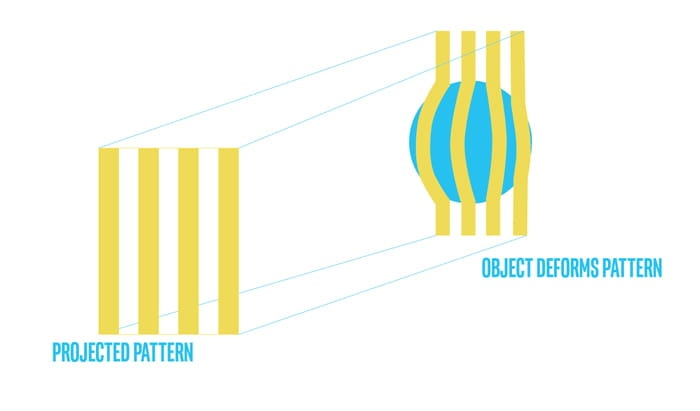
\includegraphics[width=1\columnwidth]{report1-img001.png} % Example image
	\caption{Deformation of structured light on a spherical object}
\end{figure}

\subsubsection{Stereo Depth}

Stereo depth cameras also often project infrared light onto a scene to improve the accuracy of the data, but unlike coded or structured light cameras, stereo cameras can use any light to measure depth. For a stereo camera, all infrared noise is good noise. Stereo depth cameras have two sensors, spaced a small distance apart. A stereo camera takes the two images from these two sensors and compares them. Since the distance between the sensors is known, these comparisons give depth information. Stereo cameras work in a similar way to how we use our two eyes for depth perception. Our brains calculate the difference between the images that each eye receives. Objects closer to us will appear to move significantly from eye to eye image, where an object far away would appear to move very little.

Because stereo cameras use visual features to measure depth, they will work well in most lighting conditions including outdoors. The addition of an infrared projector means that in low lighting conditions, the camera can still perceive depth details. The other benefit of this type of depth camera is that there are no limits to how many you can use in a particular space – the cameras don’t interfere with each other in the same way that a coded light or time of flight camera would.

The distance these cameras can measure is directly related to how far apart the two sensors are – the wider the baseline is, the further the camera can see. In fact, astronomers use a very similar technique to measure the distance of faraway stars, by measuring the position of a star in the sky at one point in time, and then measuring that same star six months later when the earth is at the furthest point in its orbit from the original measuring point. In this way, they can calculate the distance (or depth of the star) using a baseline of around 300 million kilometers.

\begin{figure}[h] % [h] forces the figure to be output where it is defined in the code (it suppresses floating)
	\centering
	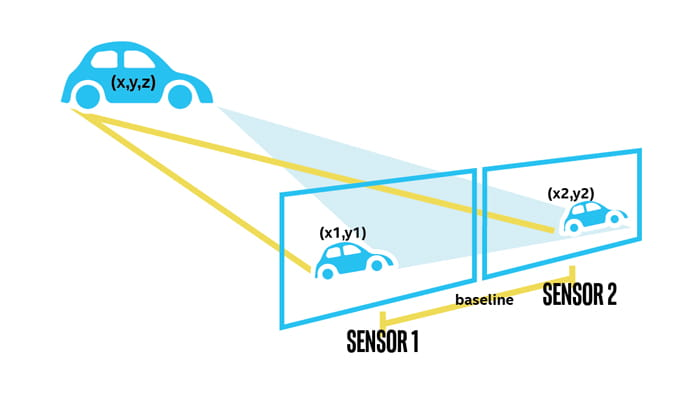
\includegraphics[width=1\columnwidth]{report1-img002.png} % Example image
	\caption{Representation of stereo depth vision}
\end{figure}


\subsection{The T265 tracking camera}

Until recent years sailors would navigate by the stars, using their movements and positions to successfully find their way across oceans. The T265 tracking camera uses a combination of cameras and Inertial Measurement Units (IMU) to navigate in a similar way, performing V-SLAM by using visual features in the environment to track it’s way around even unknown spaces with accuracy. 

The Intel RealSense T265 Tracking Camera includes two fisheye lens sensors. A fisheye lens is an ultra wide-angle lens intended to create a wide panoramic or hemispherical image. Fisheye lenses achieve extremely wide angles of view. Instead of producing images with straight lines of perspective (rectilinear images), fisheye lenses use a special mapping, which gives images a characteristic convex non-rectilinear appearance. 

.

\begin{figure}[h] % [h] forces the figure to be output where it is defined in the code (it suppresses floating)
	\centering
	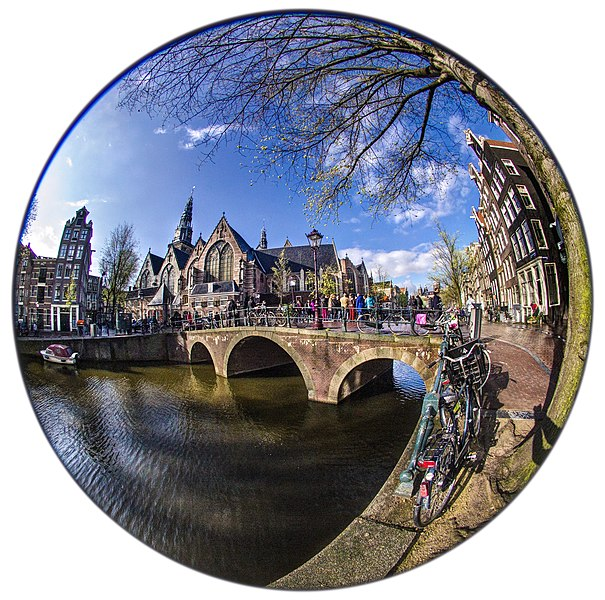
\includegraphics[width=1\columnwidth]{report1-img003.png} % Example image
	\caption{A photo taken with fisheye camera lens. The term fisheye was coined in 1906 by American physicist and inventor Robert W. Wood based on how a fish would see an ultrawide hemispherical view from beneath the water.}
\end{figure}



The camera also includes an IMU and an Intel Movidius Myriad 2 VPU. All of the V‑SLAM algorithms run directly on the VPU, allowing for low latency and efficient power consumption. The T265 has been extensively tested and validated for performance, providing under 1\% closed loop drift under intended use conditions. It also offers sub 6ms latency between movement and reflection of movement in the pose. This is fast enough for even highly-sensitive applications such as Augmented and Virtual Reality. 

\section{Method}

\subsection{Setting up the environment}

Since Ubuntu 20.04 (focal fossa) and ROS noetic were utilized for the purposes of this project, the latest versions of both of these operating systems were installed on a local machine. This machine runs on 16GB of DDR-4 RAM and an average processor. It is equipped with a dedicated Nvidia graphics card utilizing 6GB of V-RAM memory. Most of the sotftware used for the purposes of this project exploits hardware acceleration in some way. Whenever this is the case, it will be specifically stated.

\subsection{Configuring the cameras}

The first necessary step to configure the cameras is the installation of the oficcial Intel® RealSense™ SDK 2.0 for ubuntu 20.04 . It was easily and successfuly installed. Both of the cameras worked as intended while using the SDK.

It is worth noting that the T265 tracking module was experiencing fatal issues when connected to the PC via USB 3.0. The errors dissappeared when it was connected via USB 2.0. A warning stating that connection over USB 2.0 could give unreliable results was being displayed nevertheless.

\begin{figure}[h] % [h] forces the figure to be output where it is defined in the code (it suppresses floating)
	\centering
	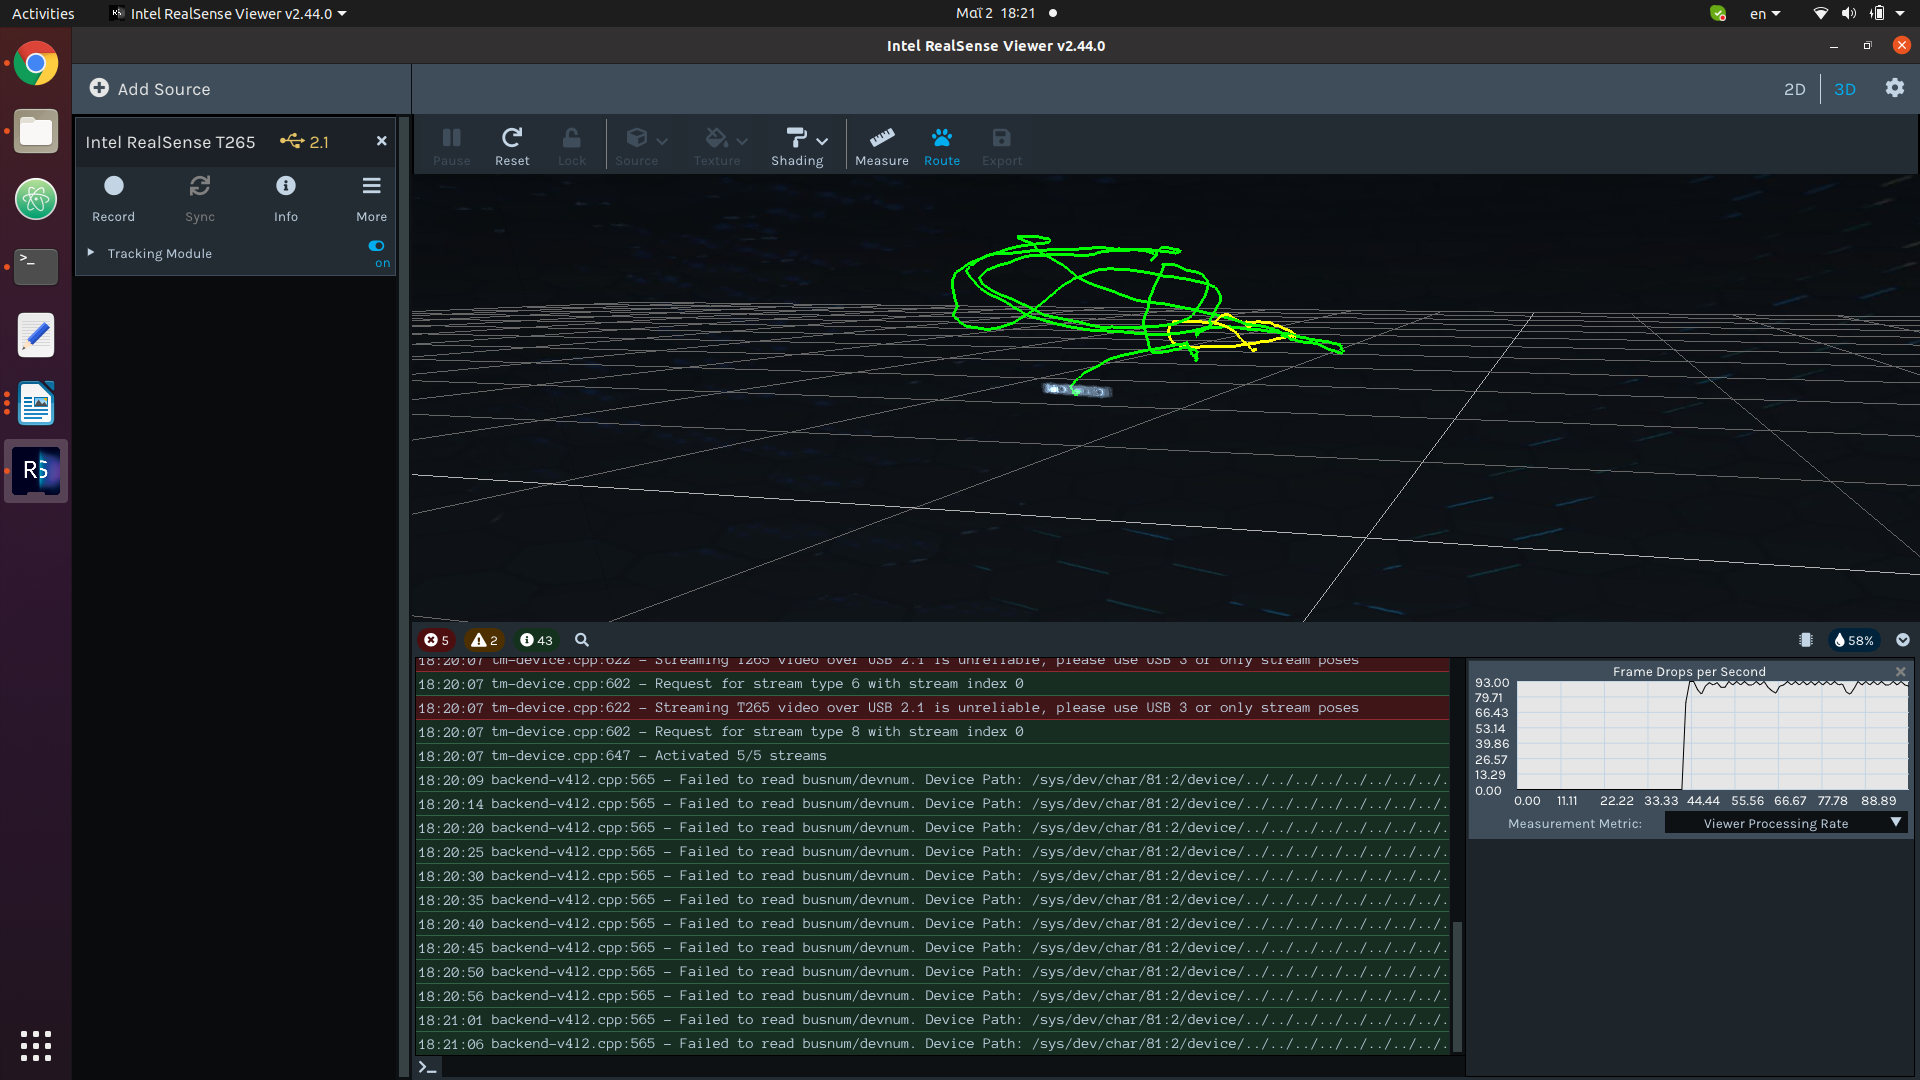
\includegraphics[width=1\columnwidth]{report1-img005.png} % Example image
	\caption{Visualizing a route calculated by the T265 tracking module, using realsense-viewer.  At the top of the image, in green, we can see the path that the module calculated during its movement. At the bottom, warnings and debug messages can be seen in red and green respectively.}
\end{figure}


The D435i camera worked as expected, providing real time depth imaging of the environment without any visible problems. The IMU module and the accelerometer were responding live to movements.

The camera was stationed 1 meter away from the base of a wooden staircase. Distances are reflected well by the depth measurement as showcased by the depth stream image. The individual stairs can be clearly distinguished in the depth image.

\begin{figure}[h] % [h] forces the figure to be output where it is defined in the code (it suppresses floating)
    \centering
	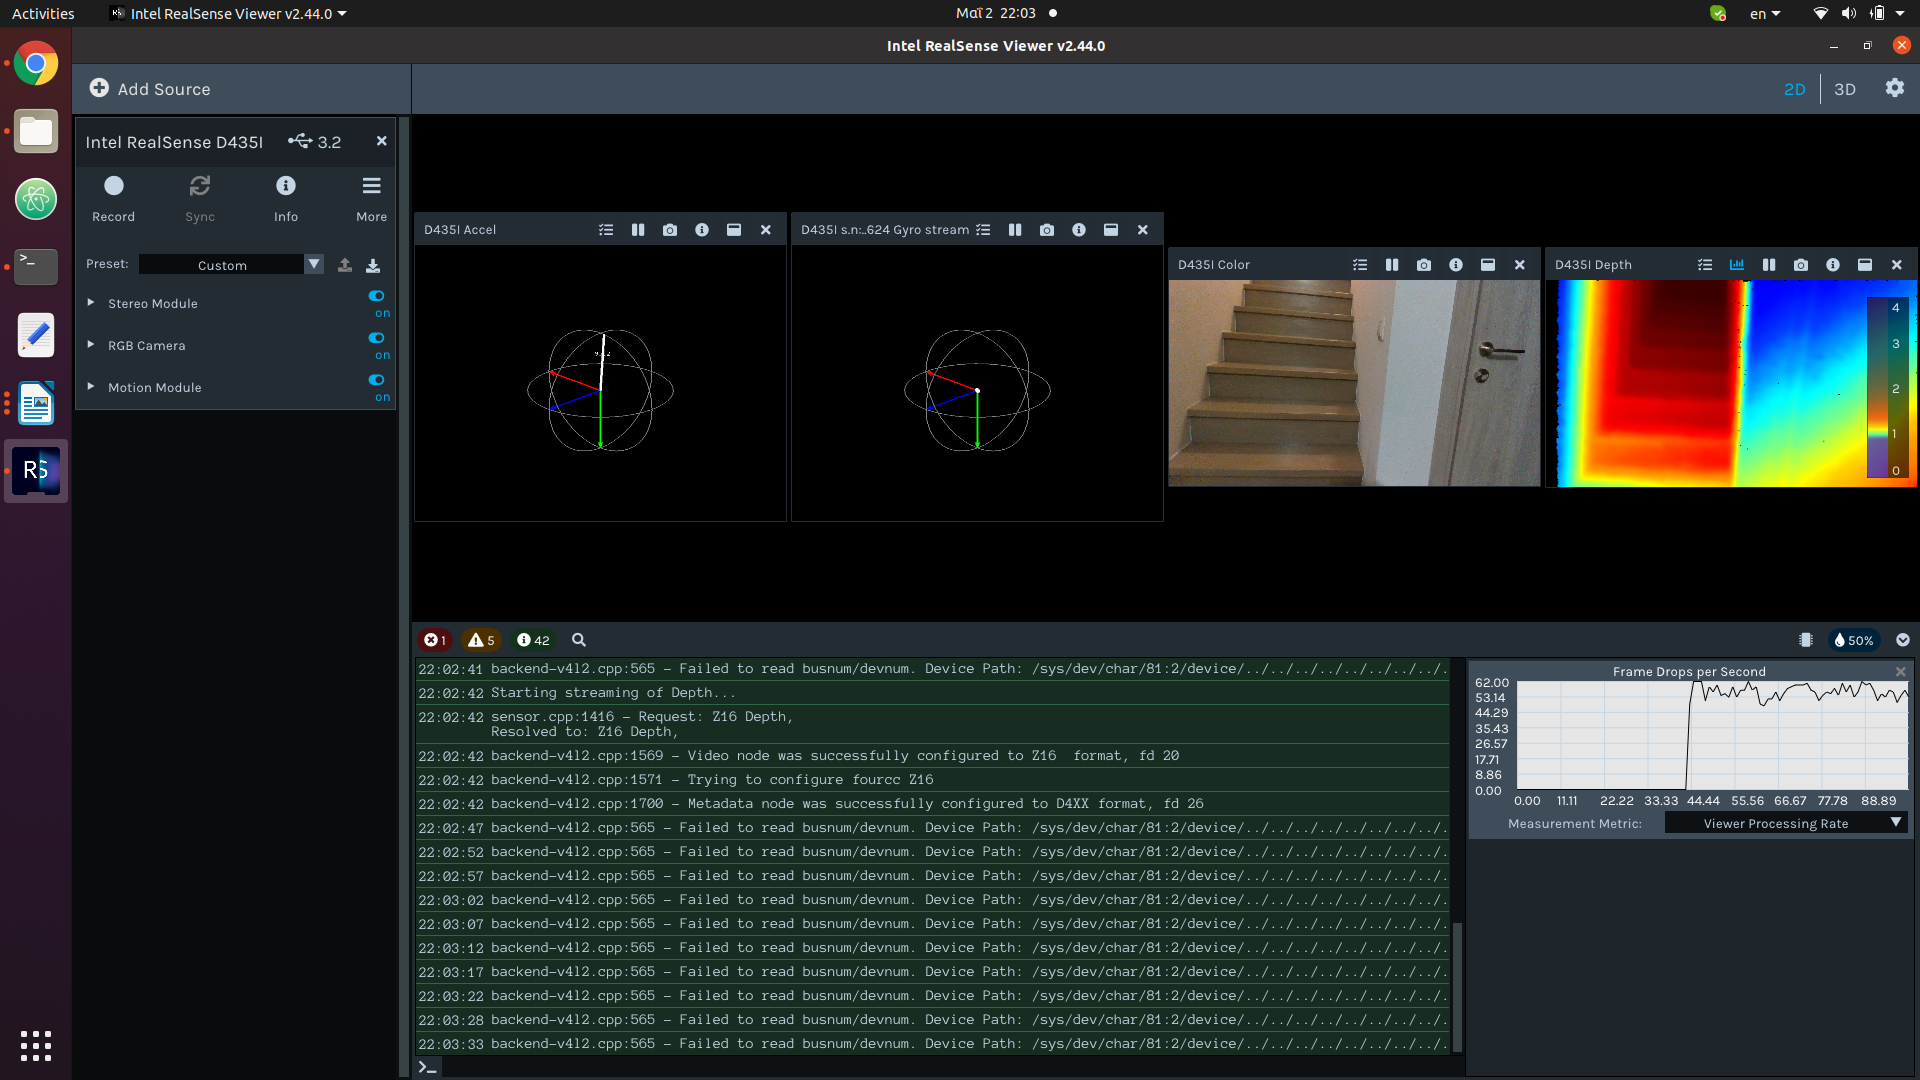
\includegraphics[width=\textwidth,height=\textheight,keepaspectratio]{report1-img006.png} % Example image
	\caption{The realsense-viewer environment with the D435i camera. At the top of the image we observe the accelerometer, gyro, color and depth streams. At the bottom debug messages can be seen in green color.}
\end{figure}

\begin{figure}[h] % [h] forces the figure to be output where it is defined in the code (it suppresses floating)
    \centering
	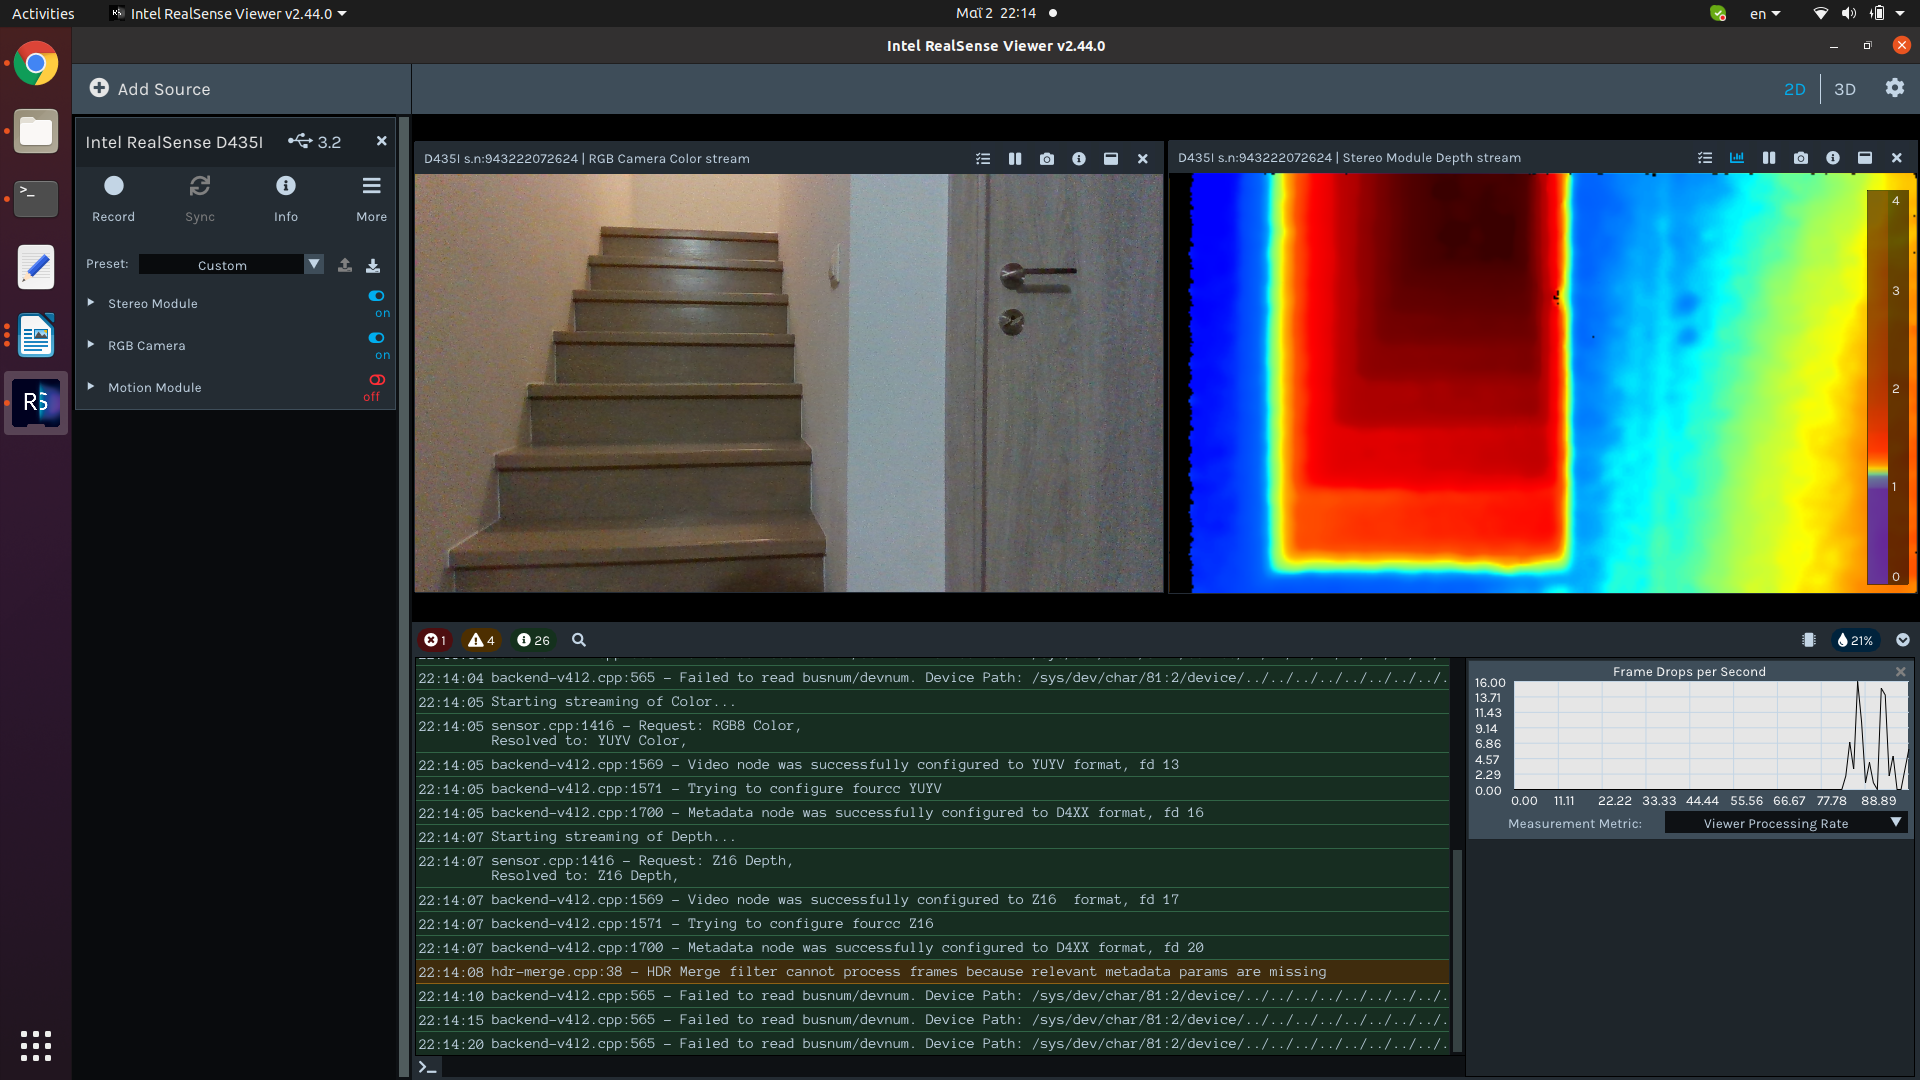
\includegraphics[width=\textwidth,height=\textheight,keepaspectratio]{report1-img007.png} % Example image
	\caption{The depth stream image of a wooden staircase. Visible on the right side of the depth image is a color scale that assigns color to depth in meters. The base of the staircase can be seen in green which means that it is registered as being 1 meter away from the camera.}
\end{figure}

\clearpage

\subsection{Installing a Ros Wrapper}

A C++ ROS Wrapper is a design pattern that uses one C++ class to expose a ROS interface for an underlying, or wrapped, piece of code. Each ROS Wrapper is instantiated inside of a ROS Node, reads its configuration from the Parameter Server, and often publishes/subscribes to information on Topics using a namespace passed to them on construction. Any number of ROS Wrappers may be instantiated within a single ROS Node and can be linked together via both their ROS interfaces and their C++ APIs.\href{http://wiki.ros.org/navigation/ROS_Wrappers}{[6]}

Regarding the ROS Wrapper for the realsense cameras, it is a way for the realsense cameras to publish data over ROS topics so that they can be used by other ROS nodes or services.
Two installation methods for the realsense ROS Wrapper are available:

The first one is installing the ROS Distribution of the wrapper and the second one is installing the Intel® RealSense™ Distribution. The first one is the simplest method. However, as stated in the installation website, the libraries installed with the ROS Distribution might be deprecated and the communication protocol used for transmitting data over ROS is less stable. \href{https://github.com/IntelRealSense/realsense-ros}{[5]}

Thus, for the purposes of this project, the  Intel® RealSense™ Distribution was installed. Note that the .travis.yml file which is in the package, should be consulted during this more elaborate installation. If the following packages are not installed or updated in your system, they should be installed/updated using:

\begin{lstlisting}[language=bash]
  $ sudo apt install "$_python"-rosdep -y
  $ sudo rosdep init
  $ rosdep update
  $ sudo apt-get install ros-$_ros_dist-cv-bridge -y
  $ sudo apt-get install ros-$_ros_dist-image-transport
  $ sudo apt-get install ros-$_ros_dist-tf -y
  $ sudo apt-get install ros-$_ros_dist-diagnostic-updater -y
  $ sudo apt-get install ros-$_ros_dist-ddynamic-reconfigure -y

\end{lstlisting}

\begin{verbatim}
Where in our case "$_python" = python3 and $_ros_dist = noetic
\end{verbatim}

Proceeding with the rest of the installation was successfull.

\subsection{First tests over ROS}

The ROS Wrapper is essentially a ROS package named realsense-ros, that can be used to work with the cameras over ROS. It includes launch files which can be used to operate a single or both of the cameras at the same time. The cameras were launched and tested first separately and then simultaneously.

During the first launch of the T265 camera, it was realised that a number of topics could not be published. The error was T265 connectivity:

\textit{[Error]: Streaming over USB 2.1 is unreliable, please use USB 3 or only stream poses.}

Considering that this issue would be reflected in the odometry topics which would later be used by our SLAM algorithms, it had to be resolved before procceeding. After several tests with the T265 tracking camera, it was realised that the camera showed unexpected glitches when connected via USB 3.0. A USB 3.0 splitter hub was ordered in order to connect both of the cameras to a correct and identical type of port. The issue persisted nevertheless. 

Eventually, it turned out that the factory cable was faulty. A  new camera cable (USB micro-B) was used and the camera worked correctly over both USB 2.0 and USB 3.0 connections.

Observing the rs\_camera.launch file which can be used for launching the D435i camera, it was observed that most of the available topics are not published by default. The arguments enable\_depth, enable\_infra1, enable\_infra2, enable\_gyro and enable\_accel should be set to true, in order to enable the most important functionalities of the D435i camera.

\begin{figure}[h] % [h] forces the figure to be output where it is defined in the code (it suppresses floating)
    \centering
	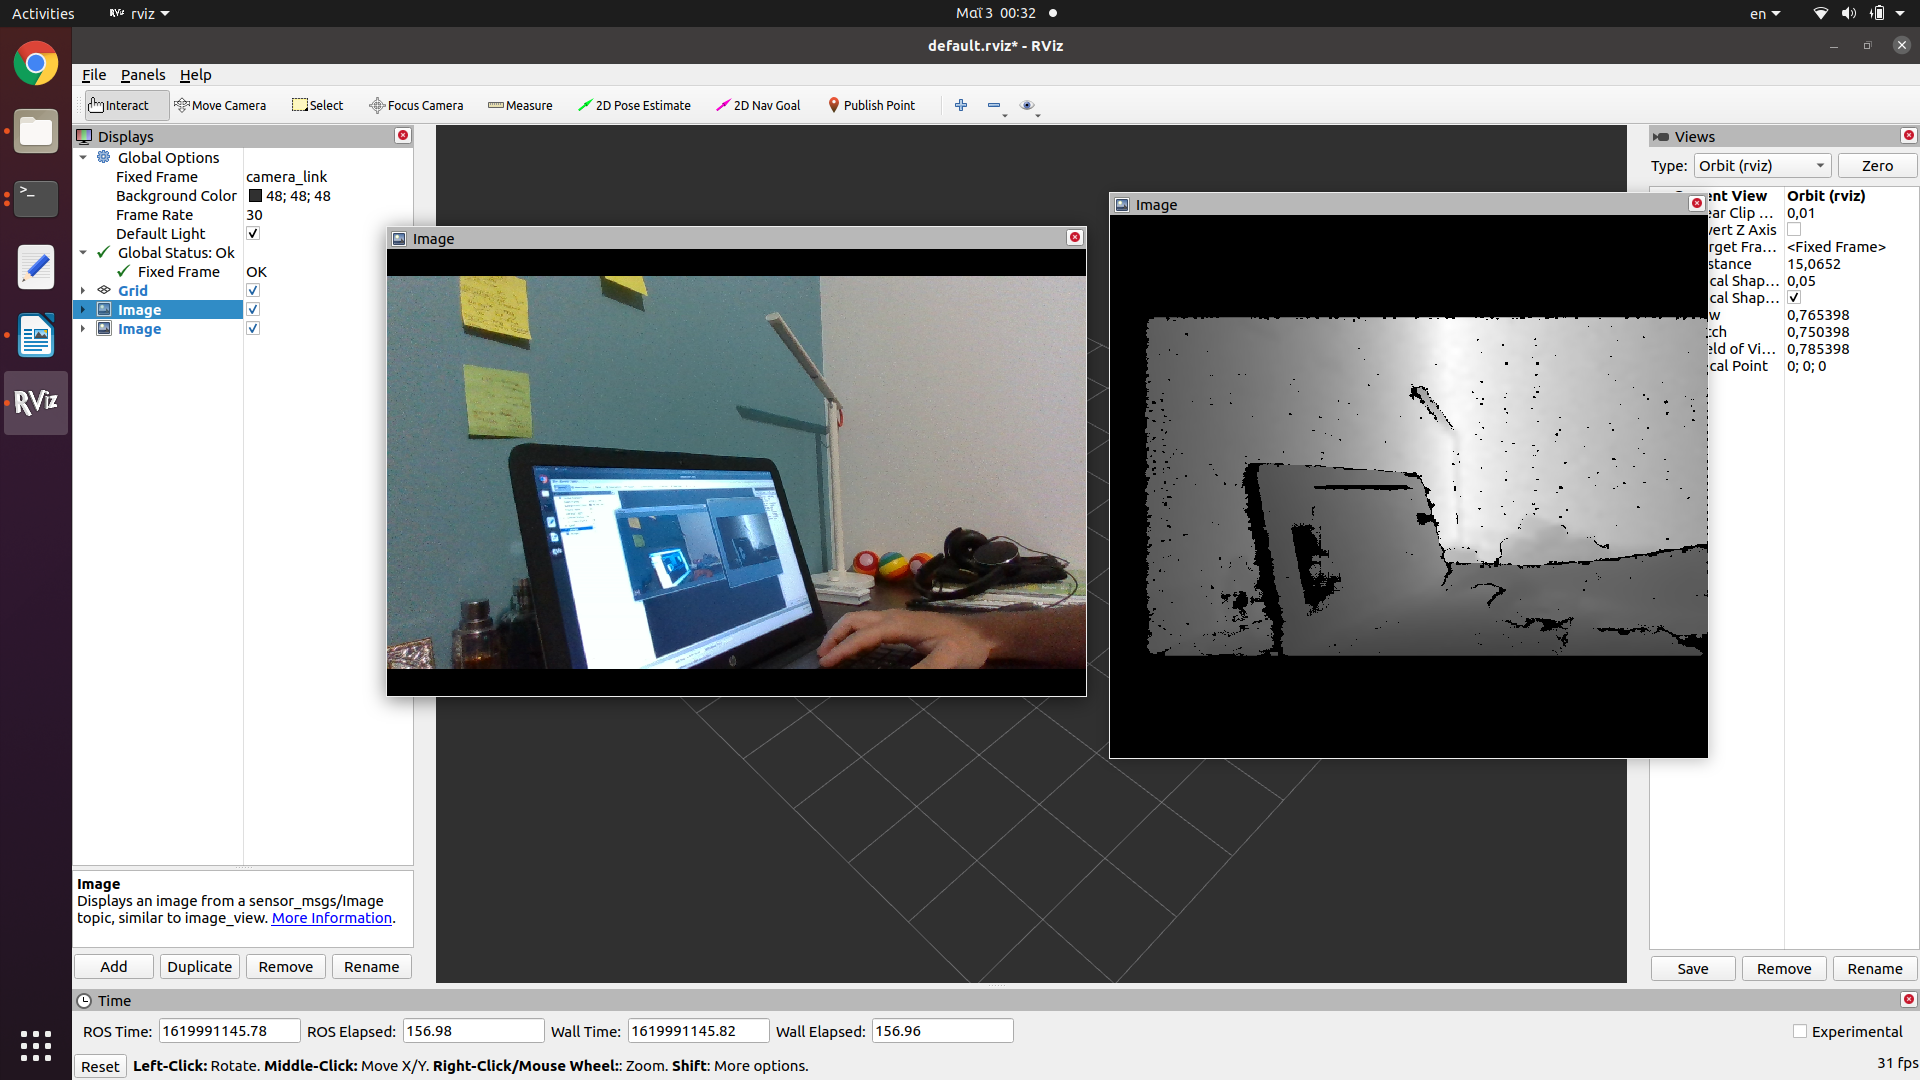
\includegraphics[width=\textwidth,height=\textheight,keepaspectratio]{report1-img008.png} % Example image
	\caption{Viewing the /color/image\_raw and /depth/image\_raw D435i topics in Rviz.}
\end{figure}

\begin{figure}[h] % [h] forces the figure to be output where it is defined in the code (it suppresses floating)
    \centering
	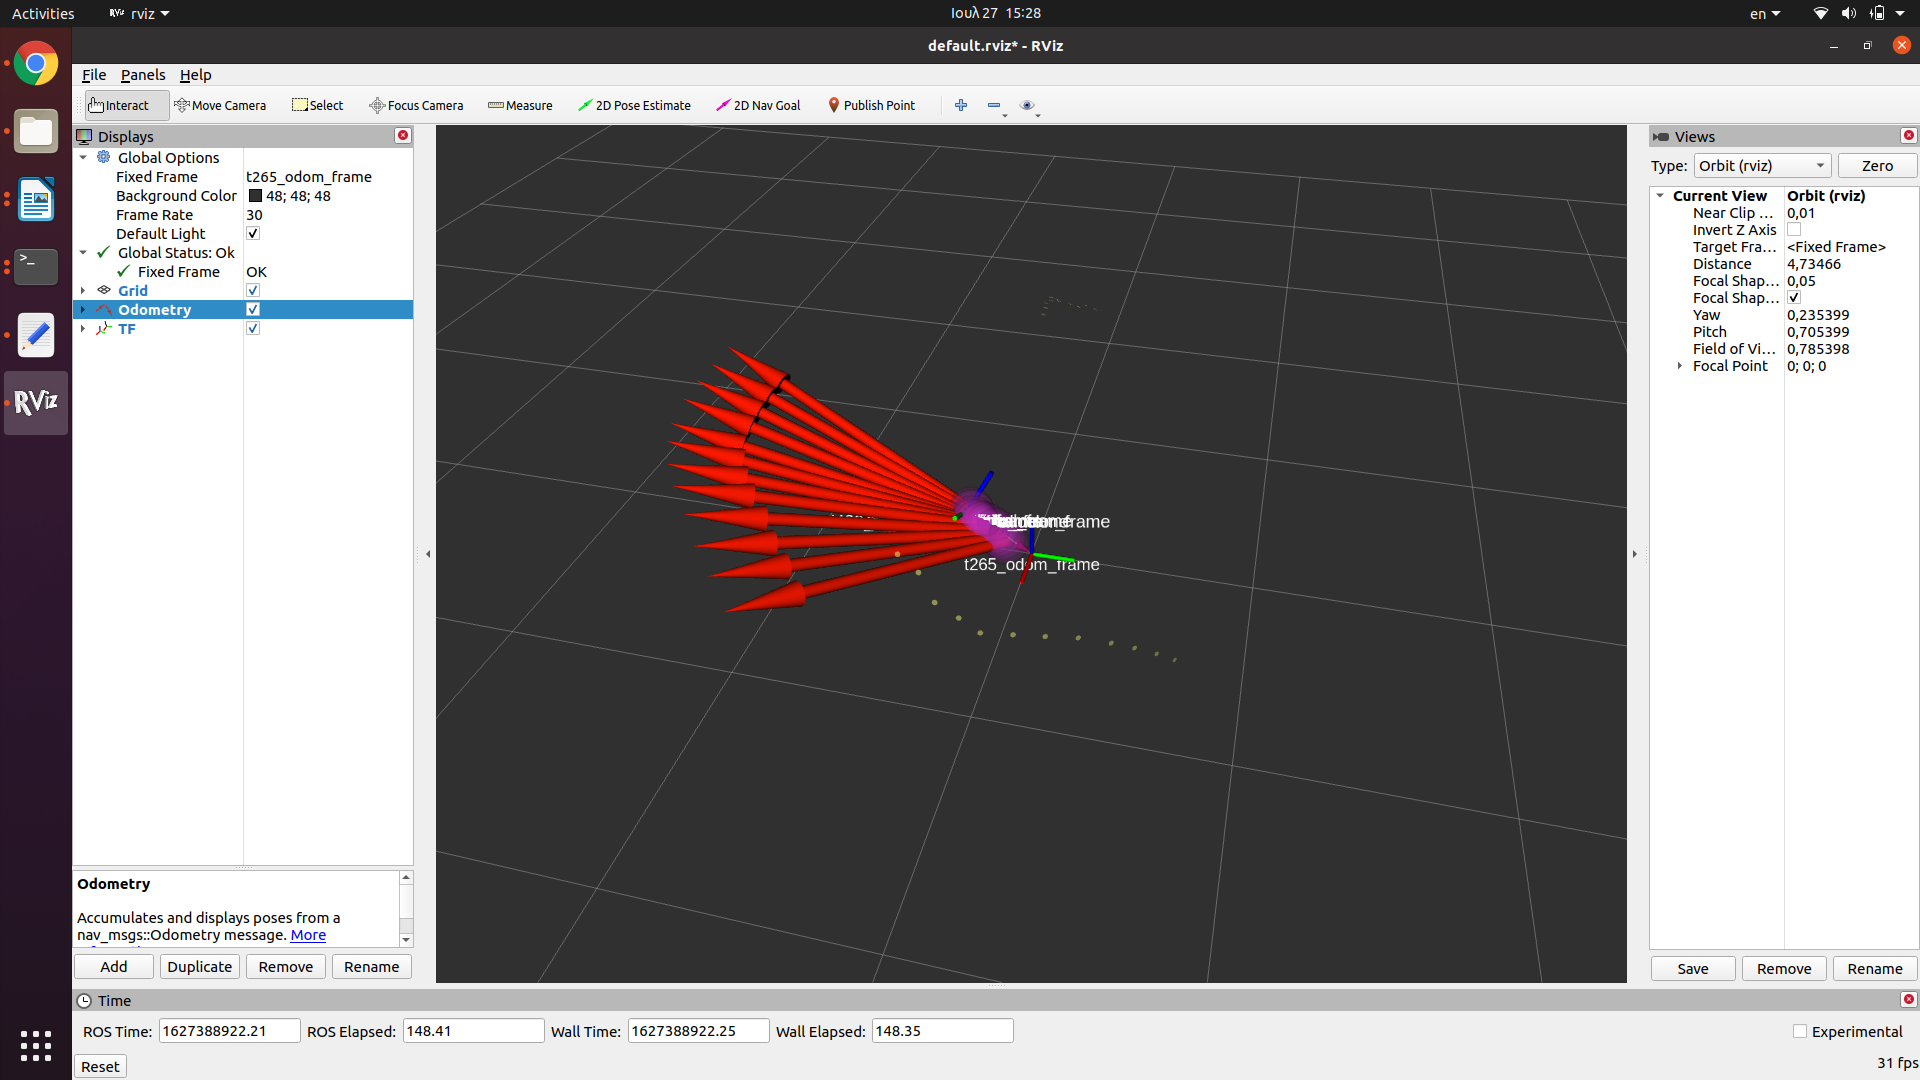
\includegraphics[width=\textwidth,height=\textheight,keepaspectratio]{report1-img009.png} % Example image
	\caption{The t265/odom/sample odometry topic. The points of the red arrows show the direction the camera faces. The arrow tail matches the camera's position over time. The purple spheres show the absolute value of the odometry covariance at each position. The little yellow dots show the orientation of the covariance.}
\end{figure}

\clearpage

\subsection{Reviewing available software packages for the Elevation Mapping}

Three different packages were tested. Each package was used to create the elevation map of a wooden staircase. The experiment took place under artificial and steady lighting conditions, indoors. The cameras were stationed 1 meter far from the base of the staircase and were handheld and moving during the tests. 

\begin{figure}[h] % [h] forces the figure to be output where it is defined in the code (it suppresses floating)
    \centering
	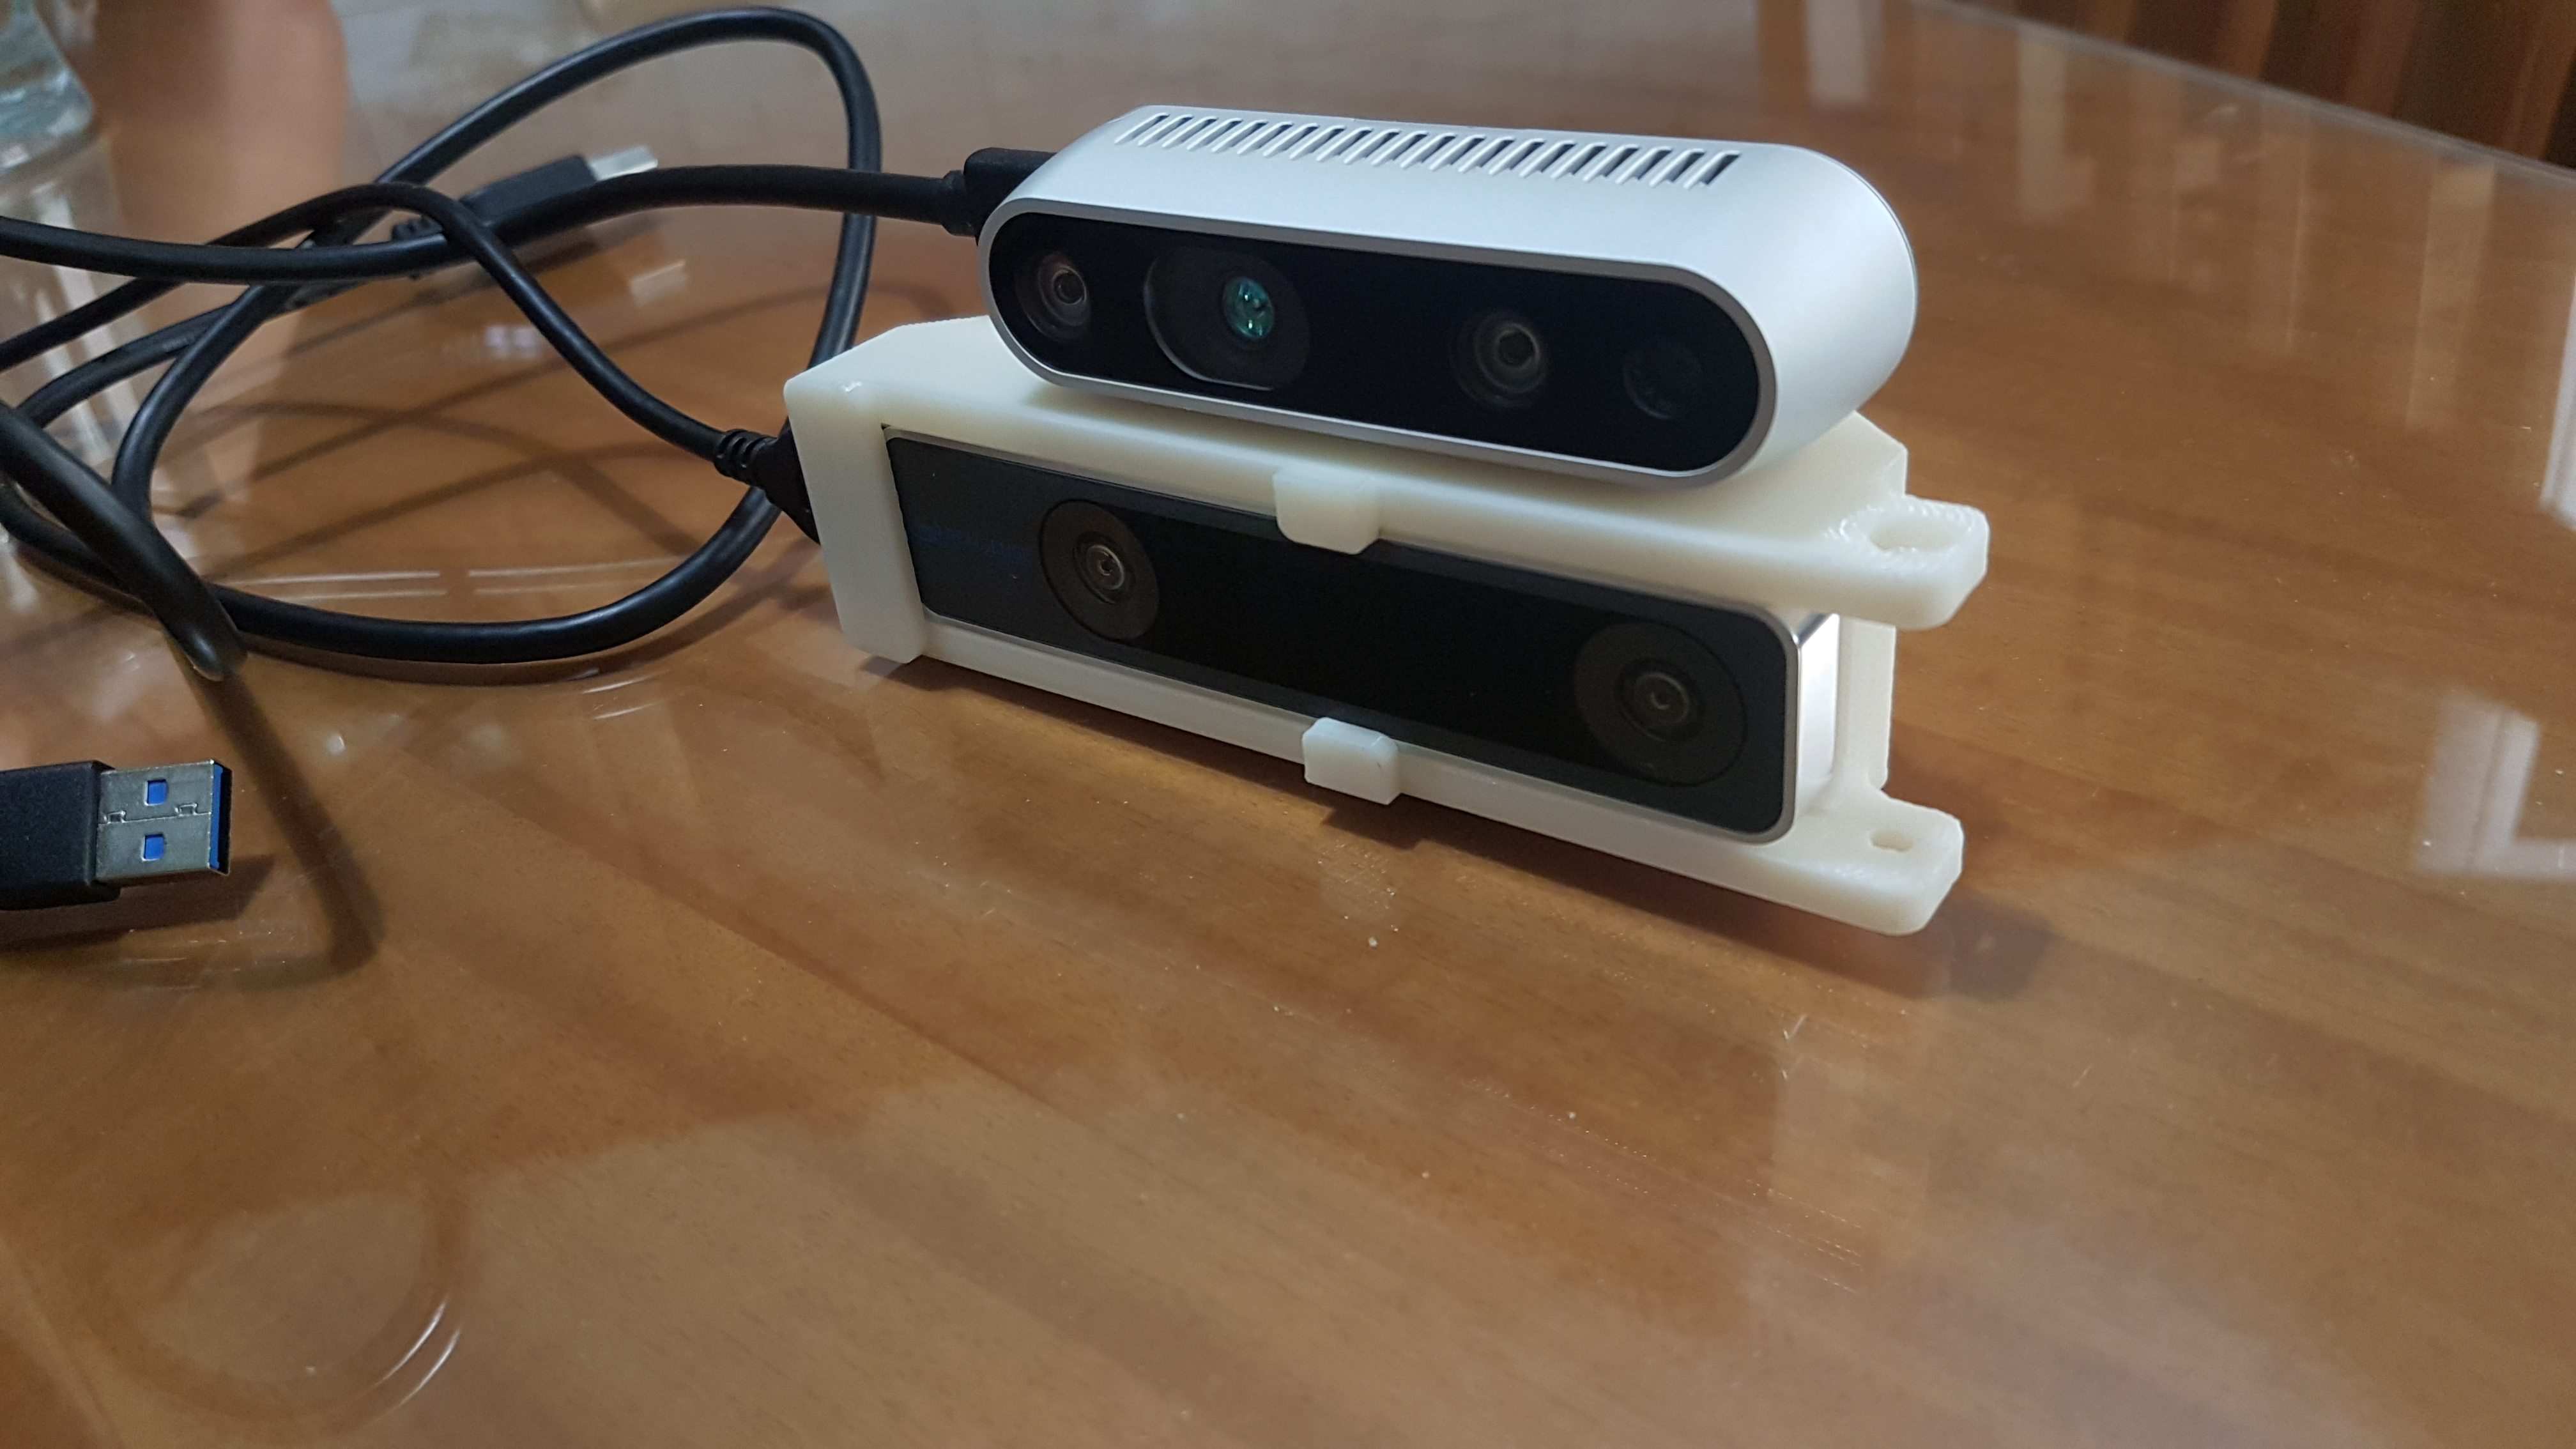
\includegraphics[width=\textwidth,height=\textheight,keepaspectratio]{report1-img010.jpg} % Example image
	\caption{The cameras were fastened on a special 3d printed mount. The static transform between the cameras corresponds to their positions on the mount.}
\end{figure}

\subsubsection{Rtabmap}

RTAB-Map (Real-Time Appearance-Based Mapping) is an RGB-D, Stereo and Lidar Graph-Based SLAM approach based on an incremental appearance-based loop closure detector. The loop closure detector uses a bag-of-words approach to determinate how likely a new image comes from a previous location or a new location. That means that each new acquired image is dissected into visual words. Similarly to how a text is dissected into words. 

For example, in the classic classification problem of labeling an email as spam or not spam, each email is parsed into words and one can deduce if the mail was spam or not spam solely by reviewing the frequency at which each word appeared. For instance, if the word “money” appeared more frequently in a target email than in the average email, then there was a large chance that the target email is spam.

Comparably, RTAB-Map parses each new frame into small homogenous pieces known as visual words. Then, it compares the frequency that each word appears in the newly acquired frame appears to a database consisting of data from previously acquired frames. If the newly acquired frame consists of similar visual words to a previously seen frame, then this bag-of-words approach determines that the new image comes from a location that has been visited before. This is known as accepting a loop closure hypothesis.

When a loop closure hypothesis is accepted, a new constraint is added to the map’s graph, then a graph optimizer minimizes the errors in the map. Namely, the information that the robot is currently in a place where it has been before is used to correct its calculated trajectory. 

A memory management approach is used to limit the number of locations used for loop closure detection and graph optimization, so that real-time constraints on large-scale environments are always respected. RTAB-Map can be used alone with a handheld stereo camera for 6DoF mapping. \href{http://introlab.github.io/rtabmap/}{[7]}

Rtabmap is a stable and well known package and can be used with structured light and stereo-depth cameras as well as with lidars and laser rangefinders. Recently, a version of the package for iOS devices has been released and produces high quality results paving the way for wider commercial use of the rtabmap algorithm. \href{https://www.youtube.com/watch?v=rVpIcrgD5c0}{[8]}

\newpage
\textit{Measuring and testing}
\bigskip

The realsense cameras along with rtabmap seem to do a very good job at producing an accurate pointcloud even when being moved vigorously while forming the map. Rviz offers a useful measurement tool. This enables the user to compare distances as perceived by the cameras with their real life counterparts. Handholding the camera at about one meter away from the base of a wooden staircase, the staircase was viewed from different angles, until an almost complete map of the staircase was generated. 

\begin{figure}[h] % [h] forces the figure to be output where it is defined in the code (it suppresses floating)
    \centering
	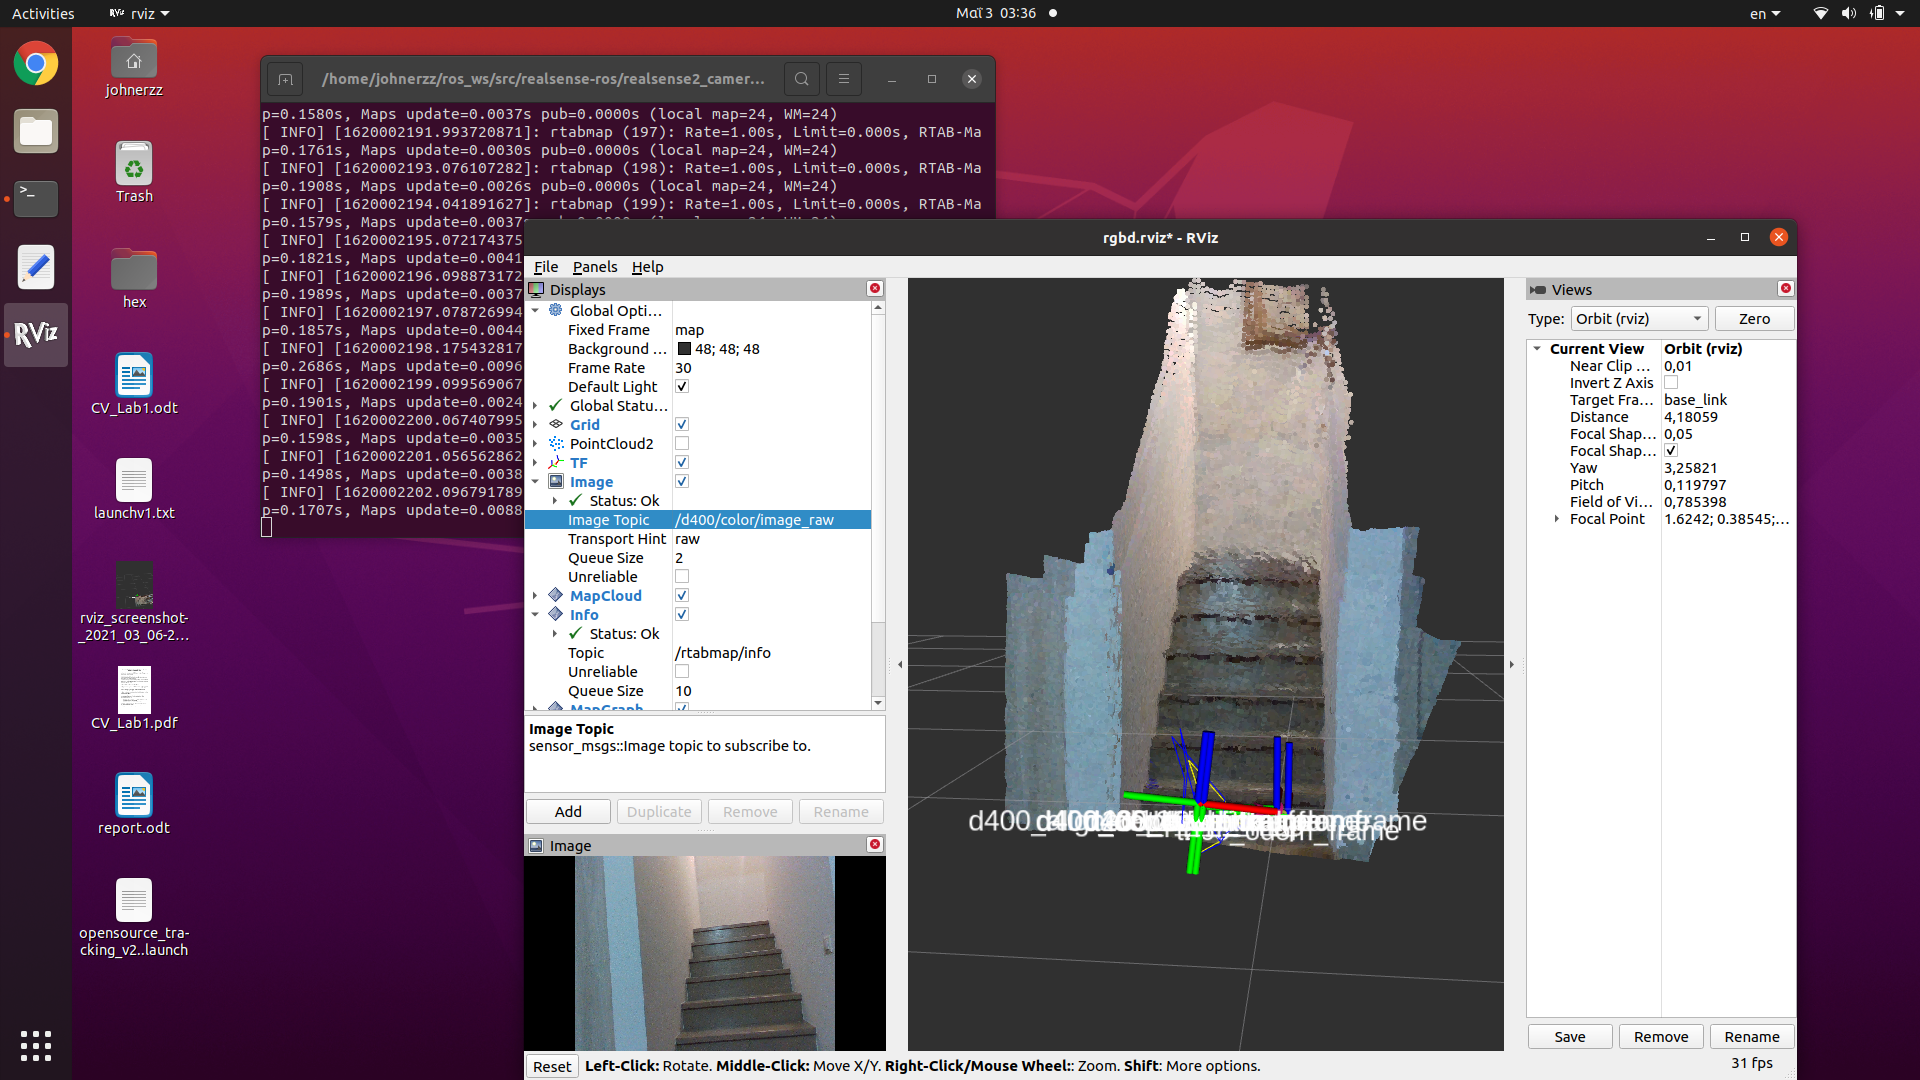
\includegraphics[width=\textwidth,height=\textheight,keepaspectratio,trim={18cm 0 4cm 8cm},clip]{report1-img011.png} %
\end{figure}

\begin{figure}[h] % [h] forces the figure to be output where it is defined in the code (it suppresses floating)
    \centering
	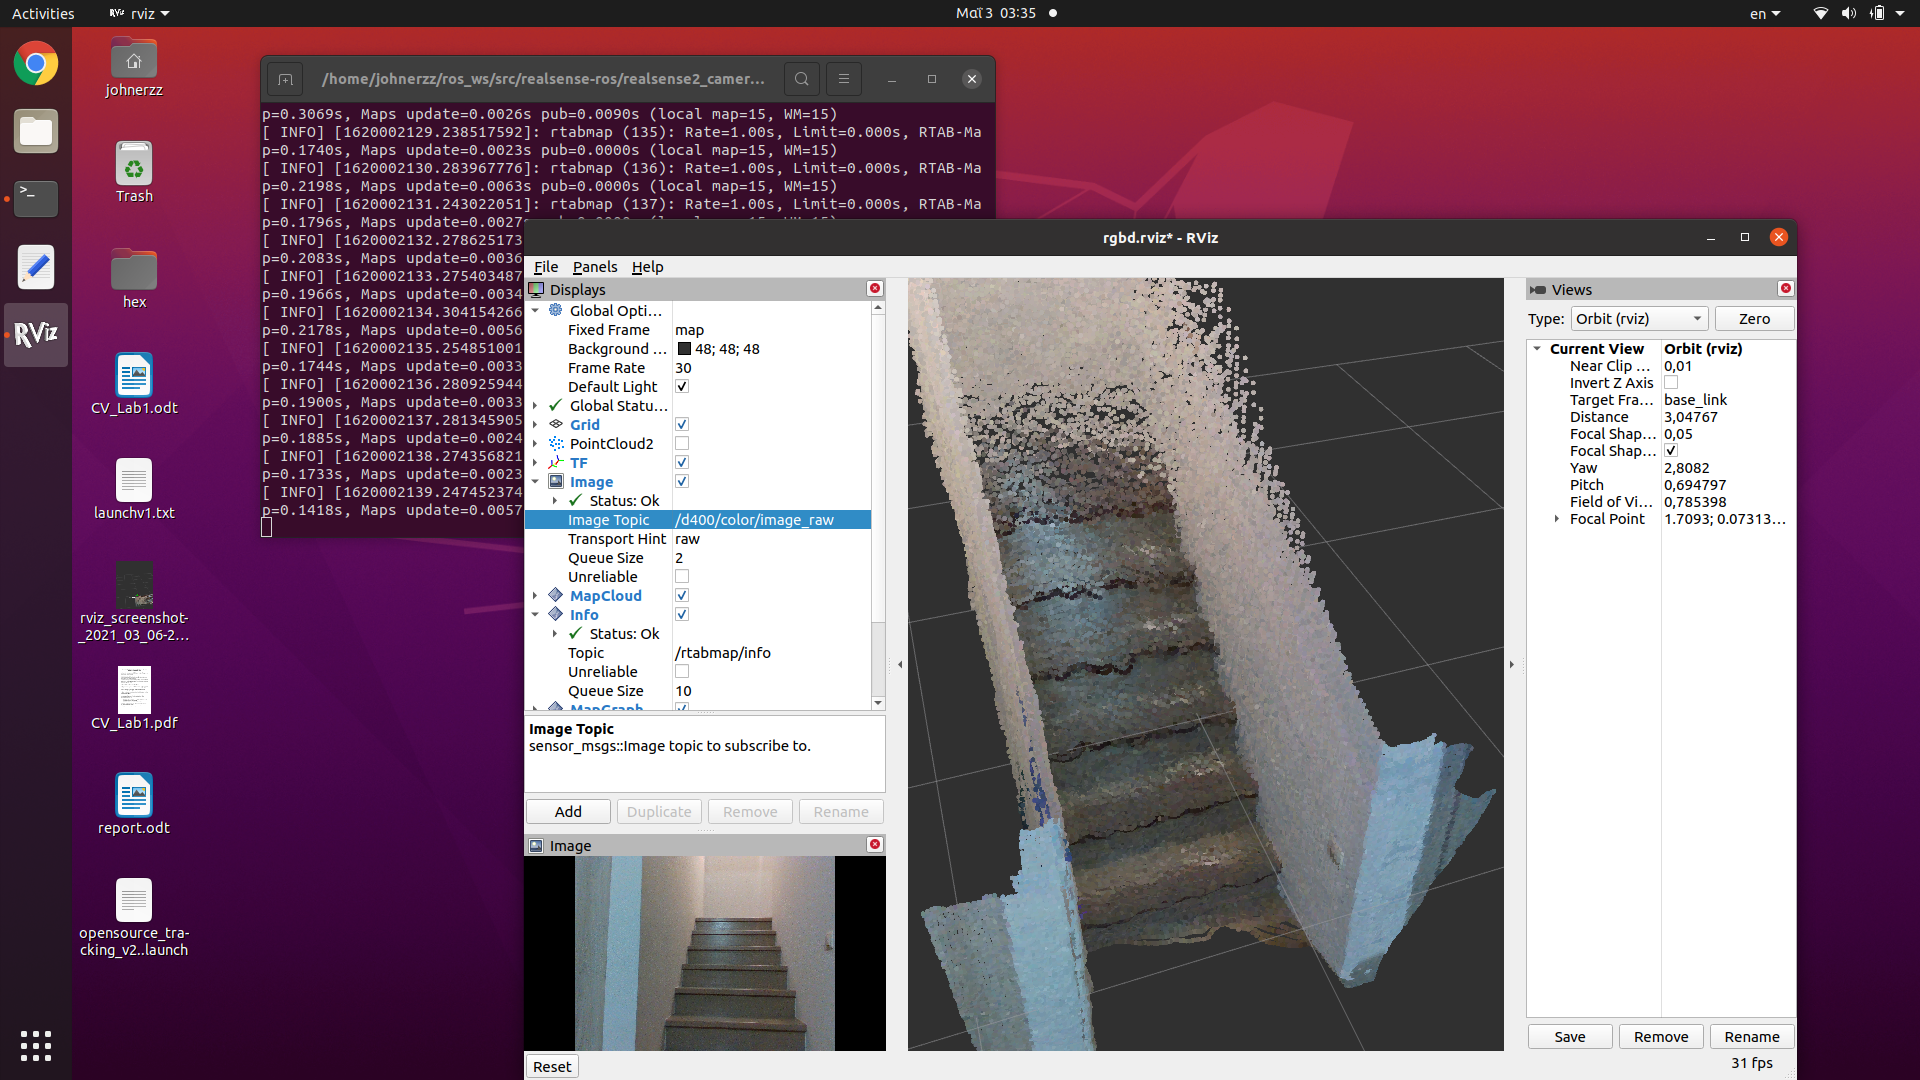
\includegraphics[width=\textwidth,height=\textheight,keepaspectratio,trim={18cm 0 4cm 8cm},clip]{report1-img013.png} %
	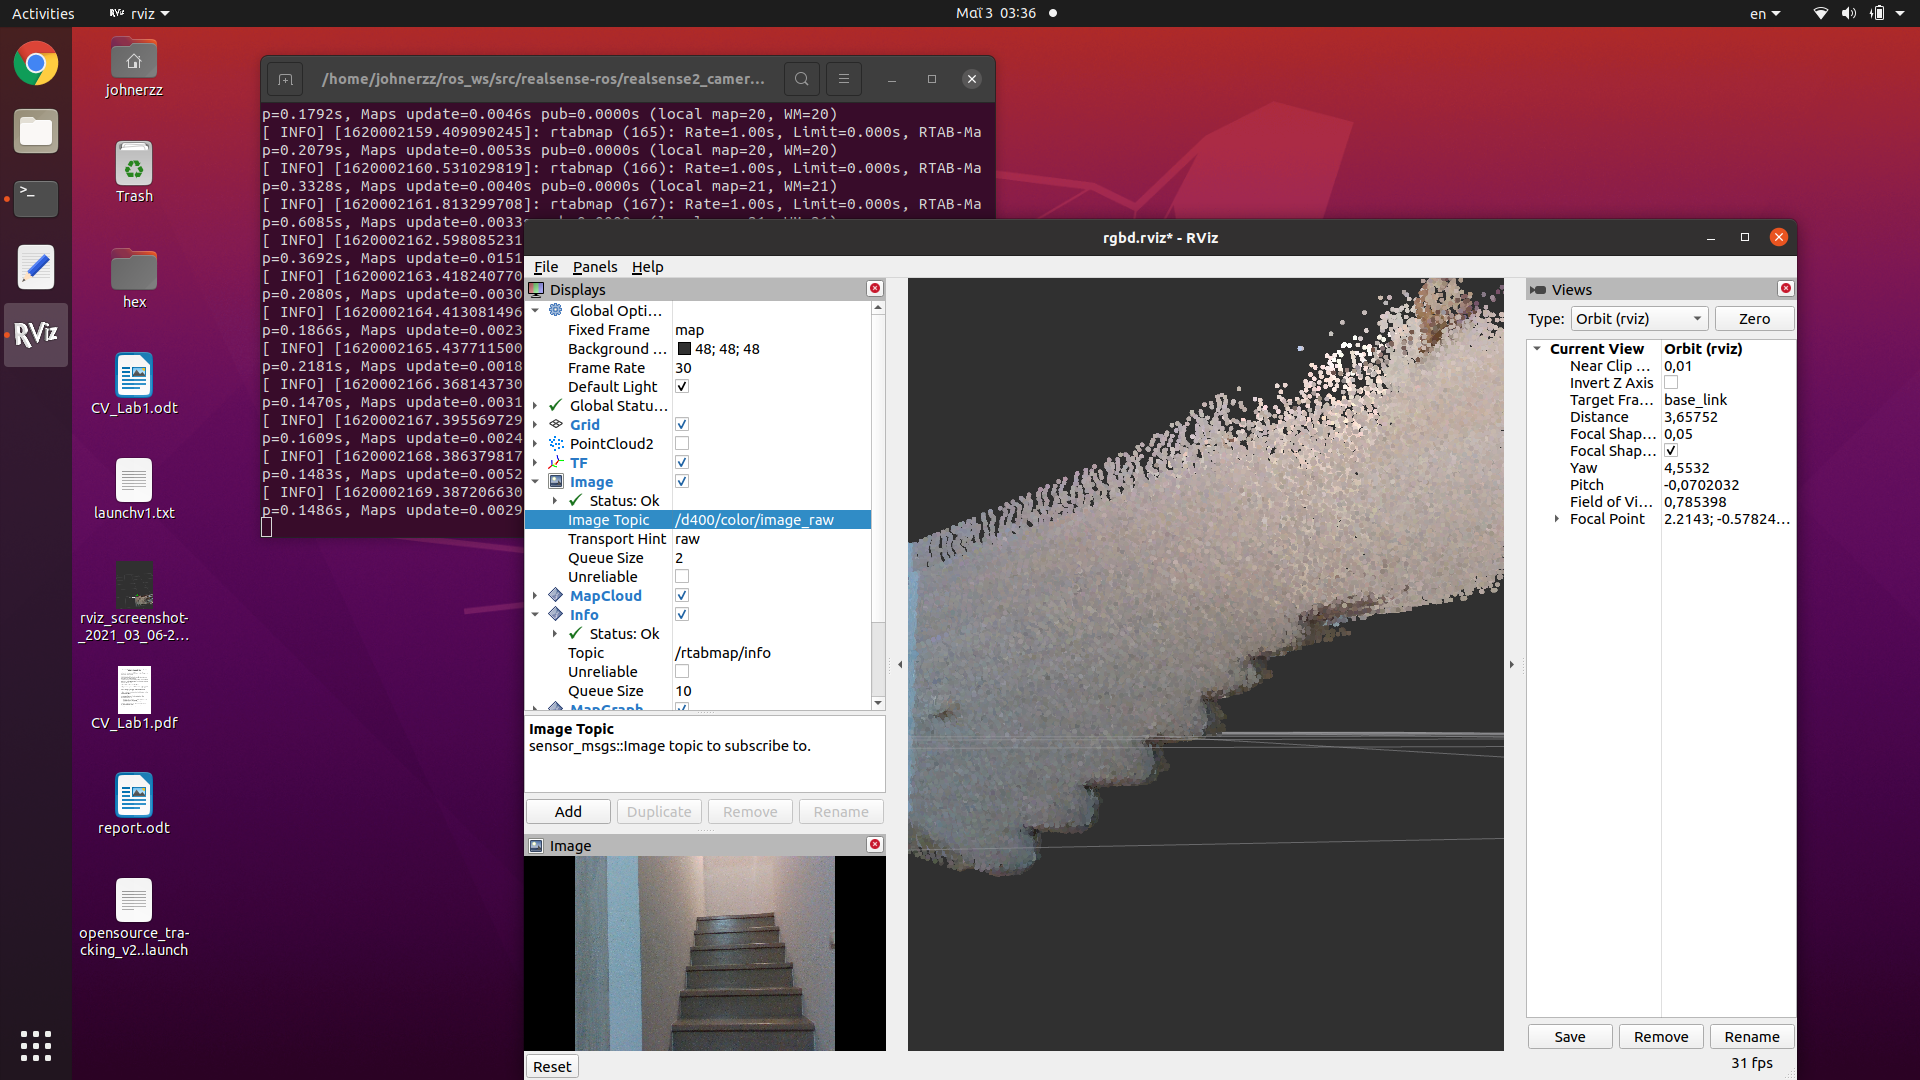
\includegraphics[width=\textwidth,height=\textheight,keepaspectratio,trim={18cm 0 4cm 8cm},clip]{report1-img012.png} %
	\caption{Elevation Mapping of a staircase made with Rtabmap. Pointcloud viewed from various angles in rviz. }
\end{figure}

\clearpage
\bigskip
\bigskip
\bigskip
\bigskip


The height of each stair step was measured as registered in the map made with rtabmap and was then compared to the real height of the stair steps which is 20cm. Subtracting the measured value from the real value gives us the measurement error. We then plot the absolute value of this error for the first six stair steps.

With an average error of about 4.6\% and given that the measurements for the real dimensions of the objects were made by hand, it can be deduced that this setup is capable of producing usable volumetric measurements. The measurements are less accurate for distant targets. This is reflected in this experiment as the fifth and sixth stair steps are measured rather inaccurately and appear noisy on the elevation map. 

\begin{figure}[h] % [h] forces the figure to be output where it is defined in the code (it suppresses floating)
    \centering
	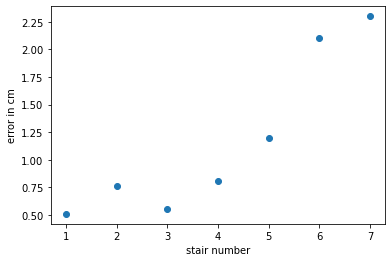
\includegraphics[width=\textwidth,height=\textheight,keepaspectratio]{report1-img014.png} %
	\caption{Absolute error value of stairs in centimeters for the first six stair steps. }
\end{figure}

\clearpage

Nevertheless, the pointcloud that Rtabmap produces with the current setup is dense and the localization of the cameras was not lost during any of our experiments. Using a detection rate of 10Hz - which means that the algorithm would check if the cameras are viewing a scene that has been viewed in the past (loop closure) ten times every second – it was observed that the node ran smoothly in real time albeit being a resource-intensive procedure. Note that there is a significant performance difference in RTAB-Map between the entire support chain (Eigen, OpenCV, VTK, and especially the feature detectors) being built with CUDA support versus without. Making use of a library that uses CUDA, is essentially using CUDA and  RTAB-Map is a package that is built with GPU acceleration in mind.

\subsubsection{Anybotics Elevation Mapping}

Anybotics Elevation Mapping is a ROS package developed for elevation mapping with a mobile robot. The software is designed for (local) navigation tasks with robots which are equipped with a pose estimation (e.g. IMU and odometry) and a distance sensor (e.g. structured light (Kinect, RealSense), laser range sensor, stereo camera). The provided elevation map is limited around the robot and reflects the pose uncertainty that is aggregated through the motion of the robot (robot-centric mapping). \href{https://github.com/ANYbotics/elevation_mapping}{[9]}

This software comes with multiple dependencies. The following software needs to be installed before installing the package itself:

\begin{itemize}
    \item Grid Map (grid map library for mobile robots)
    \item kindr (kinematics and dynamics library for robotics)
    \item kindr\_ros (ROS wrapper for kindr)
    \item Point Cloud Library (PCL) (point cloud processing)
    \item Eigen (linear algebra library)
\end{itemize}

After installing all the dependencies, the package itself was installed by cloning the latest version from the official github repository in our ROS workspace and building it according to the instructions. 

There are two tools for building ROS workspaces: catkin\_make and catkin build. The authors of the elevation mapping package proposed building with catkin build. To do that, the catkin python tools need to be installed:

\begin{lstlisting}[language=bash]
    $ sudo apt install python3-catkin-tools python3-osrf-pycommon
\end{lstlisting}

After building with catkin build, then:

\begin{lstlisting}[language=bash]
    $ roscd elevation_mapping
    $ catkin build --catkin-make-args run_tests -- --this
    $ rostest elevation_mapping elevation_mapping.test -t
\end{lstlisting}

Those tests function as a diagnostic tool to ensure that everything was installed correctly.

\bigskip

\textit{Testing in simulation}

\bigskip

Before attempting to configure the package to work with our cameras, the package was tested in a simulated environment. This makes it possible to study how the algorithm would perform with a perfect depth sensor in a noiseless environment. The turtlebot simulated robot was used in a simulated house environment.

\begin{figure}[h] % [h] forces the figure to be output where it is defined in the code (it suppresses floating)
    \centering
	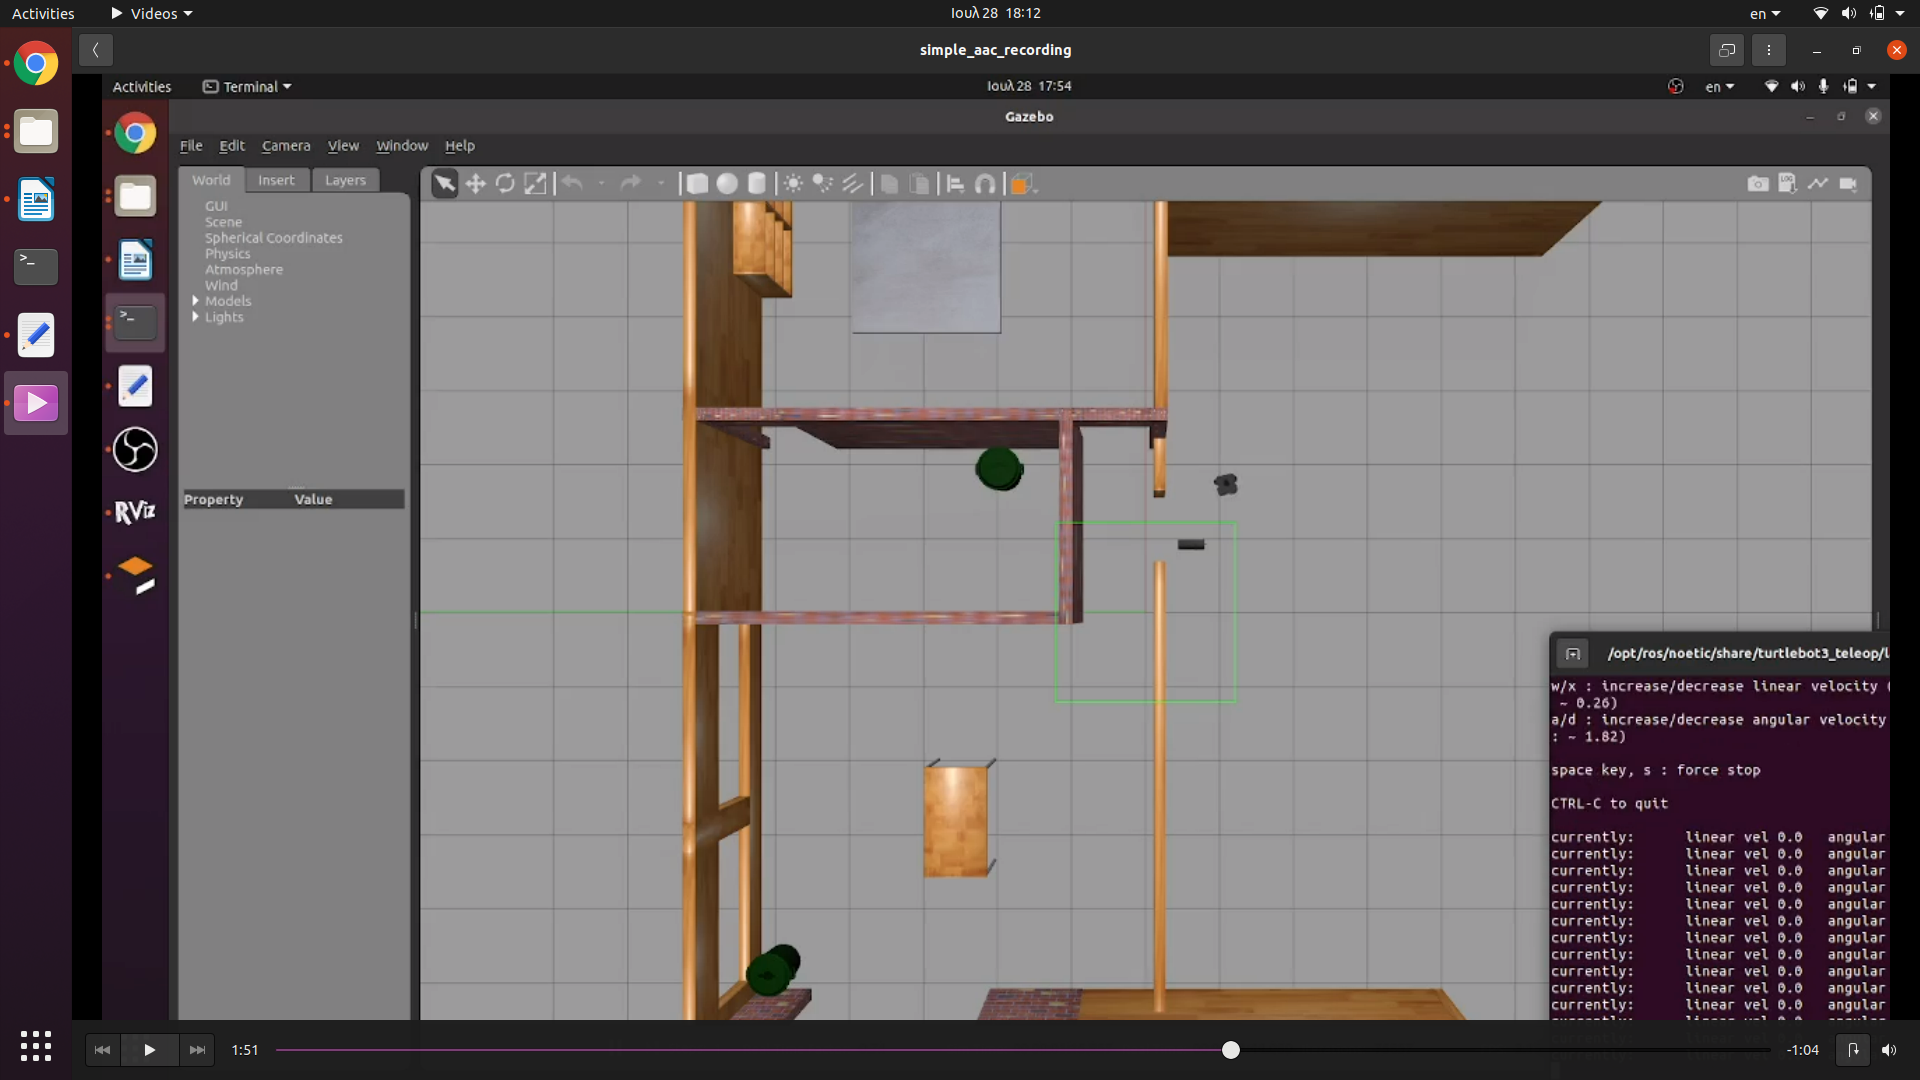
\includegraphics[width=\textwidth,height=\textheight,keepaspectratio]{report1-img015.png} %
	\caption{The simulated house environment as seen in Gazebo ROS. }
\end{figure}

The resulting map was a near perfect elevation map as was expected with a simulated setup. The map was being generated in real time in a smooth and consistent manner, but at a lower frequency than the one observed with rtabmap.

\begin{figure}[h] % [h] forces the figure to be output where it is defined in the code (it suppresses floating)
    \centering
	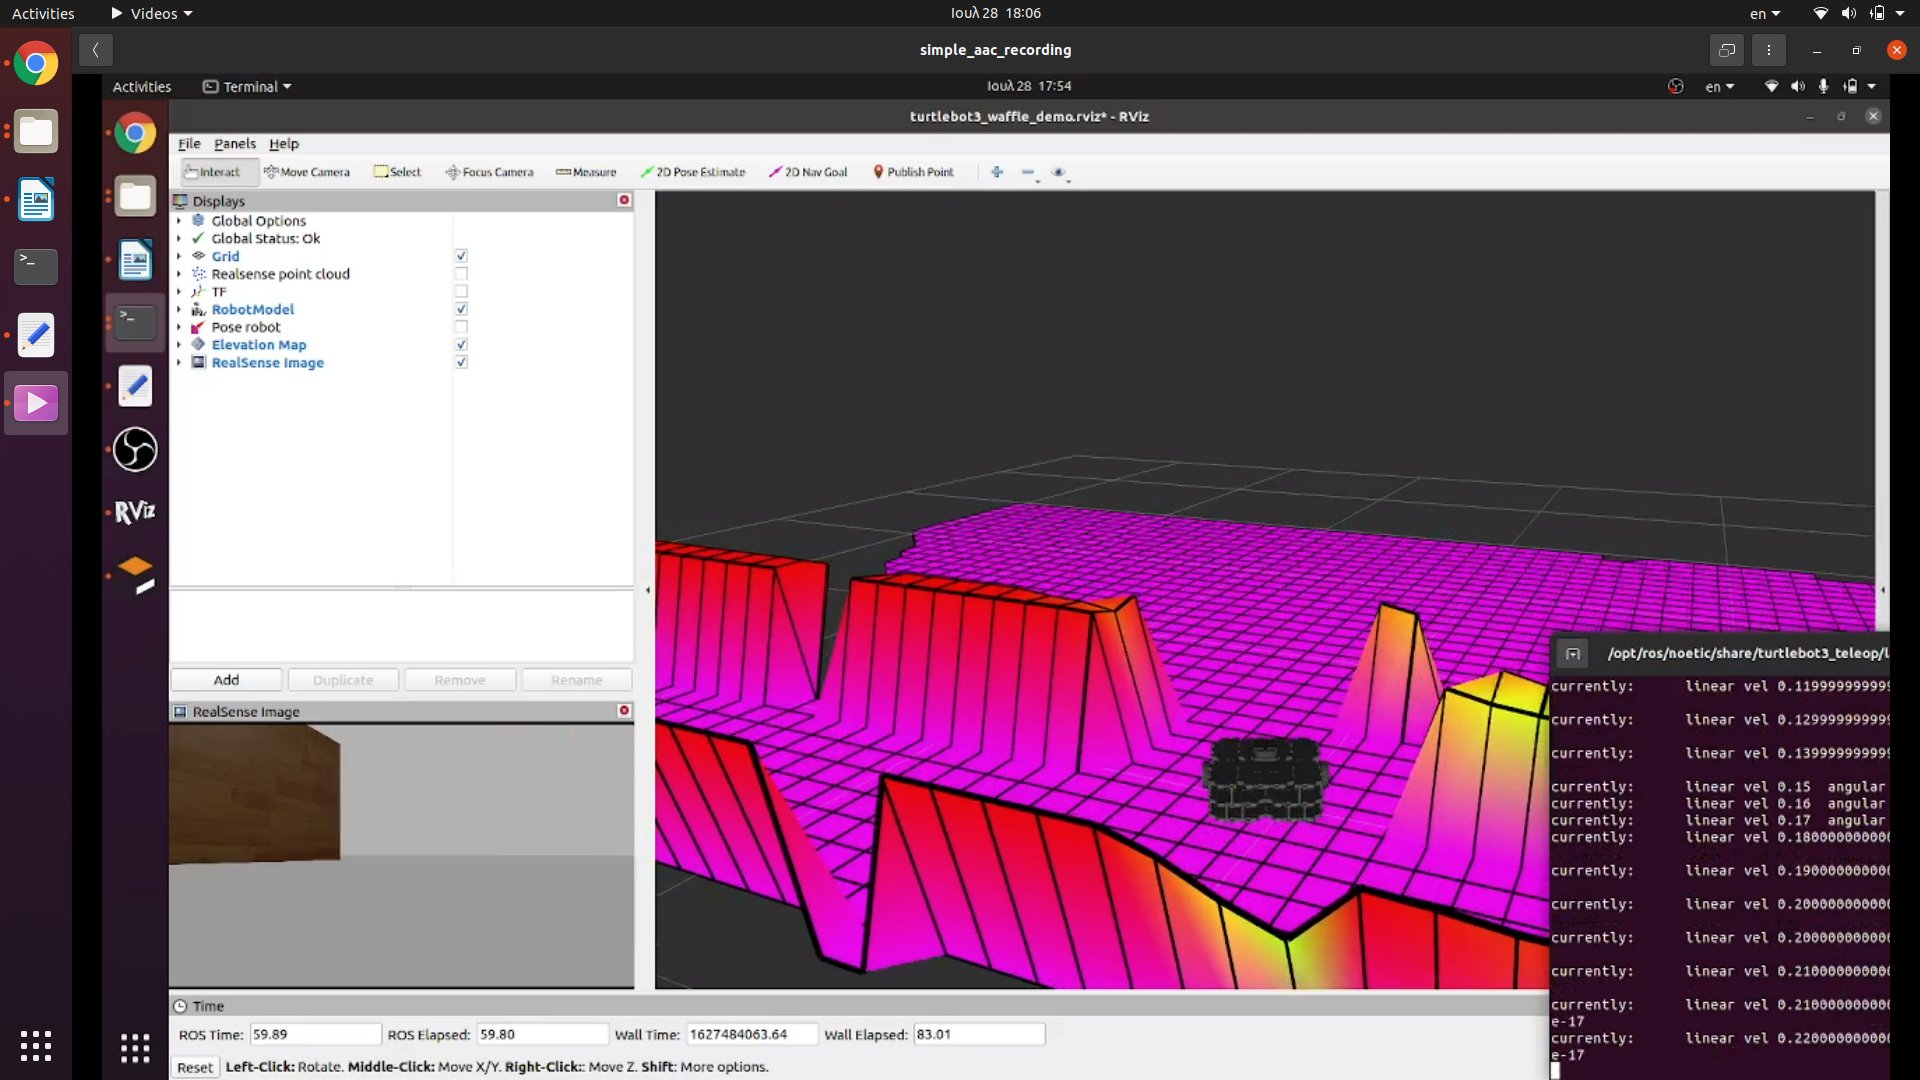
\includegraphics[width=\textwidth,height=\textheight,keepaspectratio]{report1-img016.png} %
	\caption{The elevation map of the simulated house as seen in Rviz. }
\end{figure}

\bigskip
\clearpage

\textit{Testing with the real cameras}

\bigskip

Next, the package was configured to work with the D435i and T265 cameras. A launch file was written to launch both of the cameras with the parameters required from the software. The software also required a pose instead of a TF transform so the tf\_to\_pose\_publisher.py script was used to publish the pose taken from the t265\_odom\_frame tf transform that the T265 produces. Finally Rviz is launched with the recommended arguments that were also used in the turtlebot simulated demo.

A .yaml configuration file was then written to provide the elevation mapping node with the topics and parameters it would read to generate the map. The "/d435/depth/color/points" pointcloud topic from the D435i camera and the "t265\_odom\_frame" transform topic from the T265 camera were ultimately chosen.

The first tests turned out to be noisy. It was then understood that the model had to be fed with the expected sensor noise as well as the type of depth camera used so that the elevation mapping algorithm compensates and sharpens the result. Thus, a sensor processor for the D435i camera was added. The results were visibly better.

\begin{figure}[h] % [h] forces the figure to be output where it is defined in the code (it suppresses floating)
    \centering
	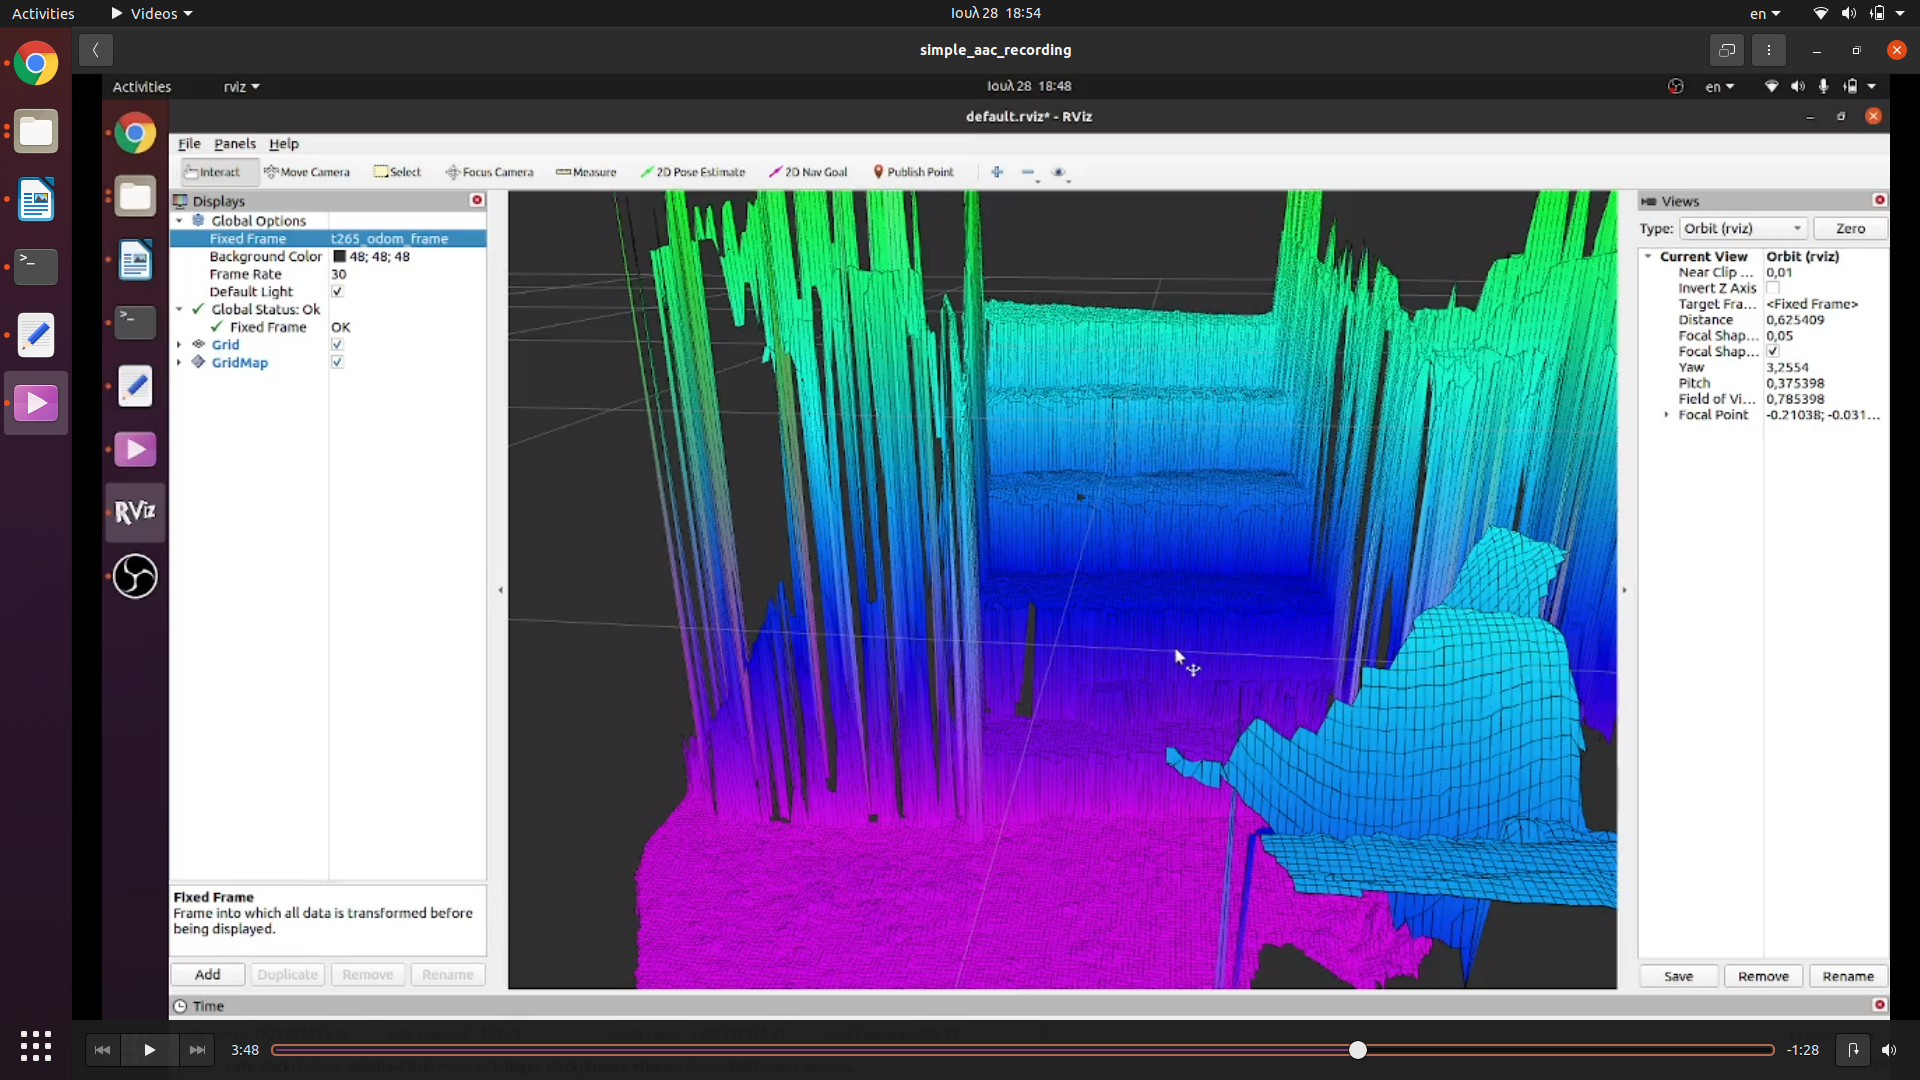
\includegraphics[width=\textwidth,height=\textheight,keepaspectratio]{report1-img017.png} %
	\caption{The chromatic elevation map of the wooden staircase as displayed in Rviz. }
\end{figure}

During the experiment of mapping the wooden staircase, it became evident that this package produces a robot-centric map. That means that in order to save computational resources (mainly memory) the map is constructed within a finite spherical space around the robot – in our case, the two cameras -. Everything outside this area will not be mapped and if the robot moves, then the spherical space moves with it, thus everything that was previously mapped but is now outside of the spherical area will be forgotten. That means that if we map the staircase but then move about three meters away from it, the stair will vanish from the map and would need to be remapped again if it was desired.

Testing the precision of this method in the same way rtabmap was tested, it is observed that this method has a similar performance. This is expected, as the accuracy of the volumetric measurements of objects is primarily affected by the camera's depth accuracy and not the software used to perform SLAM.

\begin{figure}[h] % [h] forces the figure to be output where it is defined in the code (it suppresses floating)
    \centering
	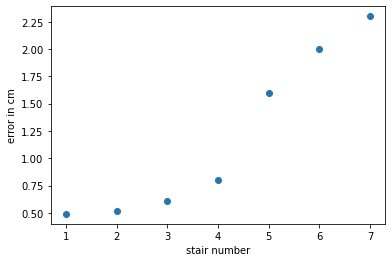
\includegraphics[width=\textwidth,height=\textheight,keepaspectratio]{report1-img018.png} %
	\caption{Absolute error value of stairs in centimeters for the first six stair steps. }
\end{figure}

Instead of just a pointcloud, this package also produces a gridmap along with an elevation scale and thus could need less processing before being used for applications such as climbing a staircase. However, this also poses drawbacks. Essentially, the map constructed with Anybotics Elevation Mapping is not a 3D map of the environment, but rather a so called 2.5D map(two-and-a-half dimensional, alternatively pseudo-3D or three-quarter): For every point in the plane on which the robot moves, we save the elevation of this point and plot the result in 3D space. This simplifies our data but also creates problems with modelling multiple surfaces that are stacked along the z-axis. For example, if we place an object 2 meters over a specific stair of the staircase, then the software will assume that the elevation at that specific area is equal to the height at which this object is, while our robot should know that there is an obstacle 2 meters over the stair, but the stair itself is not occupied and can be climbed.

\subsubsection{Gradslam}

Gradslam is a fully differentiable dense SLAM framework. It provides a repository of differentiable building blocks for a dense SLAM system. One can use these blocks to construct SLAM systems that allow gradients to flow all the way from the outputs of the system (map, trajectory) to the inputs (raw color/depth images, parameters, calibration, etc.).

Dense SLAM frameworks involve several components and most of these components are not differentiable. It is important for a framework to be fully differentiable because each of its components can then be fed into gradient based learning models. Processes such as graphics and physics are being made differentiable to embed stronger domain specific information into deep learning algorithms. This has not been the case for SLAM. Gradslam was created to provide a solution.

The latest version of pytorch was installed, as it is a prerequisite for running Gradslam. Consequently, Gradslam was installed from source and imported into a python code script to be tested.\href{https://gradslam.readthedocs.io/en/latest/tutorials/tutorial_prerequisits.html}{[10]}

\bigskip
\textit{Testing with our cameras}
\bigskip

The pyrealsense2 library was used to configure and launch the two cameras. Initially, the D435i camera was launched with the purpose of capturing a sequence of RGB-D images (colored images along with their corresponding depth image). Then, the ICL dataset format was used in order to form a gradslam-compatible dataset with the captured images. 

The script initializes RGBDdimages (a class imported from gradslam) using the newly formdd dataset and then plots the result. Next, the vertex maps and the normal maps of the staircase dataset were computed and plotted successfully. Those maps are a mathematical representation of our 3D space and in contrast to normal pointclouds they are fully differentiable.

\begin{figure}[h] % [h] forces the figure to be output where it is defined in the code (it suppresses floating)
    \centering
	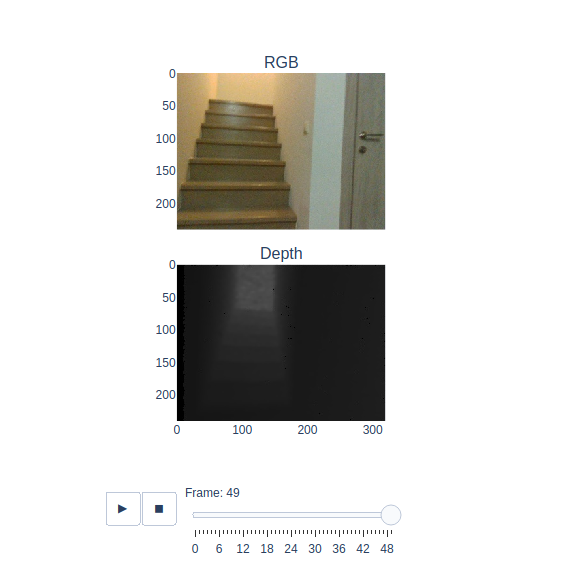
\includegraphics[width=\textwidth,height=\textheight,keepaspectratio]{report1-img019.png} %
	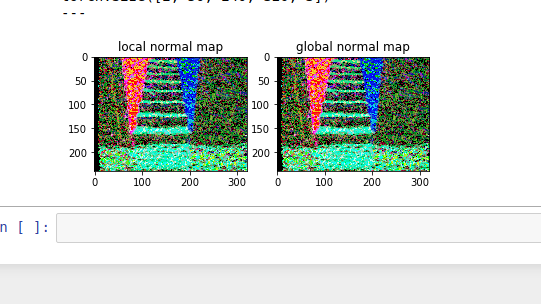
\includegraphics[width=\textwidth,height=\textheight,keepaspectratio,trim={0 4cm 0 1cm},clip]{report1-img020.png} %
	\caption{RGBDimages and vertex maps visualised. }
\end{figure}

\clearpage

Capturing pose data with the T265 camera and incorporating them into the new dataset was the next step. After formatting the data to be compatible with the ICL dataset’s format, the dataset was aggregated to achieve full SLAM. We also tested the provided step-by-step functionality in order to achieve real-time SLAM. The performance of the package was however notably slower than the performance of the packages we tested before, with the map being updated at a frequency less than 1Hz. 

The final output is comparable to what has been discussed so far. Note, however, that the aggregation of the dataset with poses received from the T265 camera, did not change the quality of the exported pointclouds at all, even when tested multiple times. We can infer that without modifications of the intrinsic software used, gradslam does not make use of the provided pose data at all. Instead, it performs visual-only SLAM (V-SLAM), which means that the algorithm estimates the orbit that the camera followed by solely reviewing the RGB-D images from the D435i camera.

\begin{figure}[h] % [h] forces the figure to be output where it is defined in the code (it suppresses floating)
    \centering
	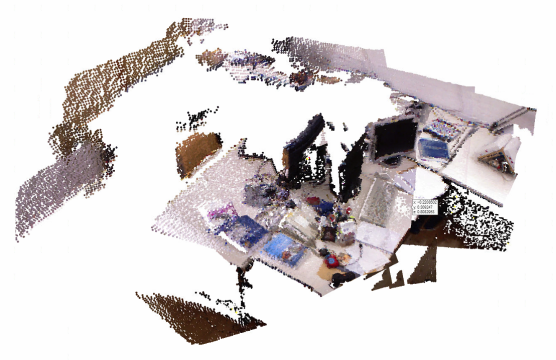
\includegraphics[width=\textwidth,height=\textheight,keepaspectratio]{report1-img021.png} %
	\caption{Pointcloud made with Gradslam on the original ICL dataset. }
\end{figure}

\subsubsection{Portability}

All of the above experiments were conducted by moving the cameras by hand while having them connected to a main laptop PC via cable. This poses a lot of constraints on the movement and the available viewing angles of the cameras. It also does not reflect the final intended use of the cameras, which is mounting them on a moving quadruped robot. 

This is to be solved by using an NVIDIA Jetson Nano module which is powered by a power bank which outputs 5V – 3A continuous current. The power was delivered via the micro USB port of the Jetson Nano

\begin{figure}[h] % [h] forces the figure to be output where it is defined in the code (it suppresses floating)
    \centering
	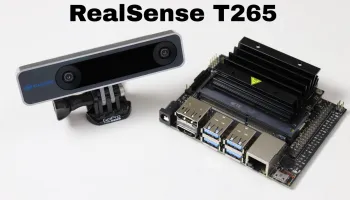
\includegraphics[width=\textwidth,height=\textheight,keepaspectratio]{report1-img022.png} %
	\caption{The realsense T265 camera alongside the Jetson Nano. }
\end{figure}


Rtabmap and Anybotics Elevation Mapping was installed on the Jetson Nano module. It was noted that it is preferable to use ros-melodic and Ubuntu 18.04 on the Jetson, because otherwise the linux kernel will require modifications for the software to run. Even so, some dependencies and libraries had to be installed manually and some of them needed to be installed in older versions to work with the Jetson Nano. 

Finally, the installed packages were tested. The results were pretty similar to those conducted on the main laptop. However, in many cases the Jetson module suddenly powered off during the experiments. In some other cases, the software would crash unexpectedly and the module would power off seconds or minutes later. The most prominent explanation is that the power supply via the micro USB port is insufficient. Various users recommend using a DC barrel jack adapter to power the Jetson Nano module. This will soon be tested. \href{https://desertbot.io/blog/jetson-nano-power-supply-barrel-vs-micro-usb}{[11]}

\newpage
[1]	“Tracking camera T265,” Intel® RealSenseTM Depth and Tracking Cameras. https://www.intelrealsense.com/tracking-camera-t265/ (accessed Jul. 29, 2021).
\bigskip

[2]	“Depth Camera D435i,” Intel® RealSenseTM Depth and Tracking Cameras. https://www.intelrealsense.com/depth-camera-d435i/ (accessed Sep. 28, 2021).
\bigskip

[3]	“Lidar cameras, Stereo Depth cameras, Coded light and Tracking cameras from Intel RealSense,” Intel® RealSenseTM Depth and Tracking Cameras. https://www.intelrealsense.com/ (accessed Oct. 02, 2021).
\bigskip

[4]	Pysource, Distance detection with Depth Camera (Intel Realsense d435i) - Opencv with Python tutorial, (2021). Accessed: Oct. 02, 2021. [Online Video]. Available: https://www.youtube.com/watch?v=mFLZkdH1yLE
\bigskip

[5]	“GitHub - IntelRealSense/realsense-ros: Intel(R) RealSense(TM) ROS Wrapper for D400 series, SR300 Camera and T265 Tracking Module.” \\ https://github.com/IntelRealSense/realsense-ros (accessed Dec. 20, 2020).
\bigskip

[6]	“navigation/ROS\_Wrappers - ROS Wiki.” \\http://wiki.ros.org/navigation/ROS\_Wrappers (accessed Jul. 29, 2021).
\bigskip

[7]	“RTAB-Map,” RTAB-Map. http://introlab.github.io/rtabmap/ (accessed Jul. 29, 2021).
\bigskip

[8]	matlabbe, RTAB-Map for iOS - LiDAR Scanner App. Accessed: Jul. 29, 2021. [Online Video]. Available: https://www.youtube.com/watch?v=rVpIcrgD5c0
\bigskip

[9]	“ANYbotics/elevation\_mapping,” Dec. 19, 2020.\\ https://github.com/ANYbotics/elevation\_mapping (accessed Dec. 20, 2020).
\bigskip

[10]	“Prerequisits — gradslam 0.1.0 documentation.”\\ https://gradslam.readthedocs.io/en/latest/tutorials/tutorial\_prerequisits.html (accessed Jul. 29, 2021).
\bigskip

[11]	“Jetson Nano Power Supply (Barrel vs. Micro USB) | desertbot.io.” https://desertbot.io/blog/jetson-nano-power-supply-barrel-vs-micro-usb (accessed Jul. 29, 2021).

\end{document}
